\documentclass[a4paper]{article}

%use the english line for english reports
%\usepackage[english]{babel}
\usepackage[portuguese]{babel}
\usepackage[utf8]{inputenc}
\usepackage{indentfirst}
\usepackage{enumerate}
\usepackage{graphicx}
\usepackage{verbatim}
\usepackage{url}


\begin{document}

\setlength{\textwidth}{16cm}
\setlength{\textheight}{22cm}

\title{\Huge\textbf{Starry Night}\linebreak\linebreak\linebreak
\Large\textbf{Programação em Logica}\linebreak\linebreak
\linebreak\linebreak

\includegraphics[scale=0.9]{img/feup-logo.png}\linebreak\linebreak
\linebreak\linebreak
\Large{Resolução de um problema de decisão}\linebreak
}

\author{\textbf{Grupo Starry Night 2:}\\ Afonso Mendonça - up201706708 \\ Filipe Nogueira - up201604129 \\\linebreak\linebreak \\
 \\ Faculdade de Engenharia da Universidade do Porto \\ Rua Roberto Frias, s\/n, 4200-465 Porto, Portugal \linebreak\linebreak\linebreak
\linebreak\linebreak\vspace{1cm}}
\date{Janeiro 5, 2020}
\maketitle
\thispagestyle{empty}

%************************************************************************************************
%************************************************************************************************

\newpage

\tableofcontents

%************************************************************************************************
%************************************************************************************************

%*************************************************************************************************
%************************************************************************************************

\newpage

\section*{Resumo}

O trabalho teve como objectivo a resolução de um problema de decisão, Starry Night, através da aplicação de restrições sobre domínios físicos e foi elaborado no âmbito da disciplina de Programação em Lógica inserida no 3º ano do Mestrado Integrado em Engenharia Informática e Computação. 

%%%%%%%%%%%%%%%%%%%%%%%%%%
\section{Introdução}

\paragraph{}
O presente trabalho centrou-se na aplicação dos conhecimentos adquiridos nas aulas teóricas e práticas de Programação em Lógica e visou a construção de um programa com capacidade para resolver um problema de decisão ou otimização em Prolog com restrições.

\paragraph{}
Com esse objectivo, foi implementada uma aplicação para encontrar soluções para o puzzle Starry Night. O puzzle tem estrutura em tabuleiro com igual número de linhas e colunas, e o seu preenchimento consiste na atribuição de ‘1’ (estrela), ‘2’ (lua) e ‘3’ (sol).

\paragraph{}
O artigo enuncia o problema e apresenta a metodologia utilizada na obtenção das soluções. No artigo ainda são vertidas as funções responsáveis pela representação das soluções e as estatísticas relativas ao processo de obtenção da solução. 

%%%%%%%%%%%%%%%%%%%%%%%%%%
\section{Descrição do problema}

Starry Night é um puzzle criado por Erich Friedman. Este puzzle é constituído por uma grelha e três símbolos distintos: um círculo branco (sol), um círculo preto (lua) e uma estrela. Para atingir a solução de deste puzzle é necessário colocar um sol, uma lua e uma estrela em cada linha e coluna da grelha. Não é permitido símbolos idênticos se tocarem na diagonal. Um círculo ao lado da grelha representa a cor do círculo mais próximo à estrela. Uma estrela ao lado da grelha significa que ambos os círculos se encontram à mesma distância da estrela. Desta forma, Starry night é um problema de decisão. O algoritmo desenvolvido é capaz de encontrar uma solução para qualquer grelha criada de dimensão igual ou superior a 5x5.

\begin{center}
    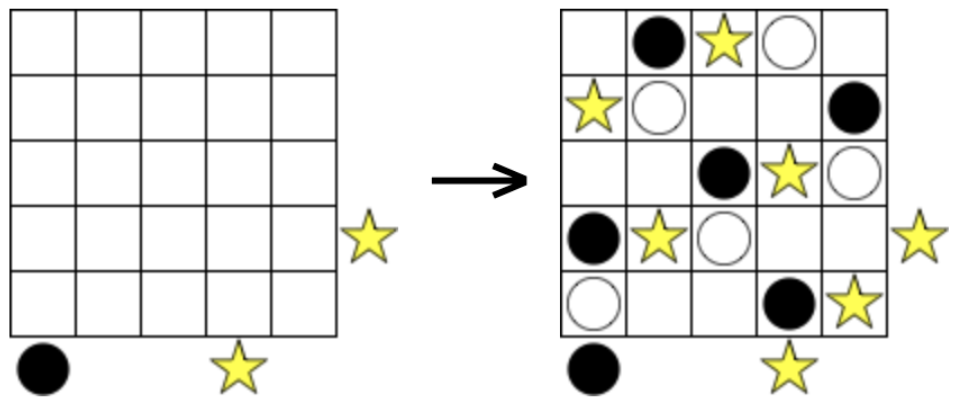
\includegraphics[scale=0.4]{img/1.png}
\end{center}

%%%%%%%%%%%%%%%%%%%%%%%%%%
\section{Abordagem}
\paragraph{}
Para encontrar uma solução para o problema exposto, recorremos à metodologia inerente à resolução de problemas de satisfação de restrições PSR.
Foram definidas variáveis de decisão e respectivos domínios bem como as restrições que limitam os valores que as variáveis podem assumir.

\paragraph{}
As soluções encontradas correspondem à atribuição a cada variável de decisão dum valor único que respeite as restrições definidas.

\paragraph{}
No problema em análise às variáveis de decisão (células do tabuleiro) pode ser atribuído o símbolo sol, lua ou estrela. As restrições incluídas no programa ditam que em cada coluna e linha do tabuleiro existe um e só um símbolo sol, lua e estrela. Na célula diagonal adjacente a uma célula, não pode existir um símbolo igual ao símbolo que consta dessa célula. Segundo as restrições definidas pelo utilizador, este define, por linha e coluna, a posição relativa dos símbolos sol e lua em relação ao símbolo estrela como anteriormente explicitado.

%%%%%%%%%%%%%%%%%%%%%%%%%%
\subsection{Variáveis de Decisão}

\paragraph{}
Considerando que a dimensão dos tabuleiros é NxN, o número de variáveis de decisão, correspondentes às células do tabuleiro, é igual a NxN. As variáveis de decisão podem assumir os valores 1, 2 e 3. Aos valores 1, 2 e 3 correspondem, respectivamente, os símbolos sol, lua e estrela.

\paragraph{}
Inicialmente, a todas as células do tabuleiro é atribuído o domínio de 0 (célula vazia). Na fase de labeling (geração da solução), é atribuído a algumas células, a solução 1, 2 ou 3, de acordo com as restrições impostas pelo utilizador.

%%%%%%%%%%%%%%%%%%%%%%%%%%
\subsection{Restrições} 

\paragraph{}
No âmbito no SICStus Prolog foram definidas como restrições rígidas as restrições descritas anteriormente quanto à obrigatoriedade de em cada linha e coluna existir um e só um símbolo sol, lua e estrela, bem como a impossibilidade de repetir na célula diagonal adjacente a cada célula, o símbolo que consta nessa célula. 

\paragraph{}
No nosso problema aos símbolos sol, lua e estrela correspondem valores quantitativos de 1, 2 e 3 respectivamente. Os predicados desenvolvidos para garantir as restrições rígidas foram os seguintes:

\subsubsection{check lines:}
Neste predicado, é garantido que o somatório de cada linha e cada coluna é igual a 6. A cardinalidade de cada linha e coluna garante que os números 1, 2 e 3 figuram uma e só uma vez.

\subsubsection{check row diagonals:}
Neste predicado é garantido que as células diagonais, à esquerda e à direita de uma determinada célula, não podem assumir um valor igual ao atribuído a essa célula.

\paragraph{}
No âmbito do mesmo programa foram assumidas restrições flexíveis introduzidas pelo utilizador que, tal como referido anteriormente, se reportam à posição, por linha e coluna, dos símbolos sol e lua relativamente ao símbolo estrela. 

\subsubsection{enforce side restrictions:}
Existem três variações deste predicado para o sol (1), lua (2) e estrela (3). É calculado um delta para os símbolos sol e lua que representam a distância relativa à estrela. No primeiro caso, o delta do sol tem que ser menor que o delta da lua. No segundo caso, o contrário, e no terceiro caso, estes últimos tem que ser iguais. Assim, neste último caso, garante-se a equidistância.

%%%%%%%%%%%%%%%%%%%%%%%%%%
\subsection{Estratégia de Pesquisa} 

\paragraph{}
Para encontrar a solução foi utilizada a estratégia de opção por omissão, ou seja, leftmost, step, up e satisfy:

\paragraph{}
labeling( [], FTB) --
[] é o mesmo que: [leftmost, step, up, satisfy].

\subsubsection{Ordenação de Variáveis:}
leftmost : variável mais à esquerda.

\subsubsection{Seleção de Valores:}
step: escolha binária entre X \#= B e X (not)\#= B, onde B é a lower ou upper bound de X.

\subsubsection{Ordenação de Valores:}
up: domínio explorado por ordem ascendente.

\subsubsection{Soluções a Encontrar:}
satisfy: todas as soluções são enumeradas por backtracking.

%%%%%%%%%%%%%%%%%%%%%%%%%%
\section{Visualização da Solução}

\paragraph{}
Ao inicializar o programa, é necessário inserir “start.” na consola. De seguida o utilizador irá deparar-se com o menu principal:

\begin{center}
    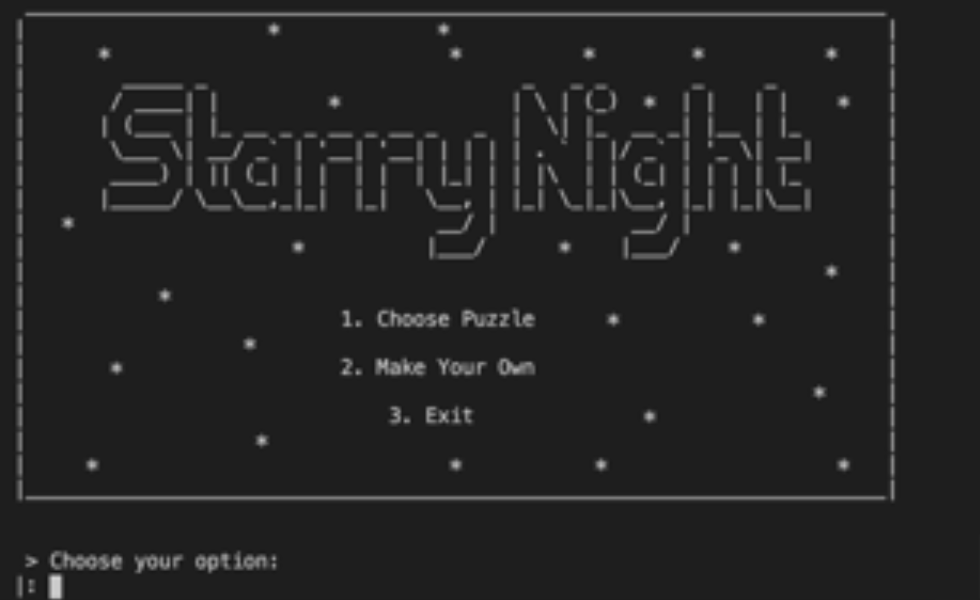
\includegraphics[scale=0.4]{img/2.png}
\end{center}

\paragraph{}
Deste ponto, o utilizador poderá escolher um dos 16 puzzles guardados (1), criar o seu próprio puzzle (2) ou sair do jogo (3).

\paragraph{}
Ao selecionar a primeira opção, o utilizador é redirecionado para o ecrã abaixo apresentado, onde o predicado "show puzzle menu" é inicializado com o primeiro puzzle.

\begin{center}
    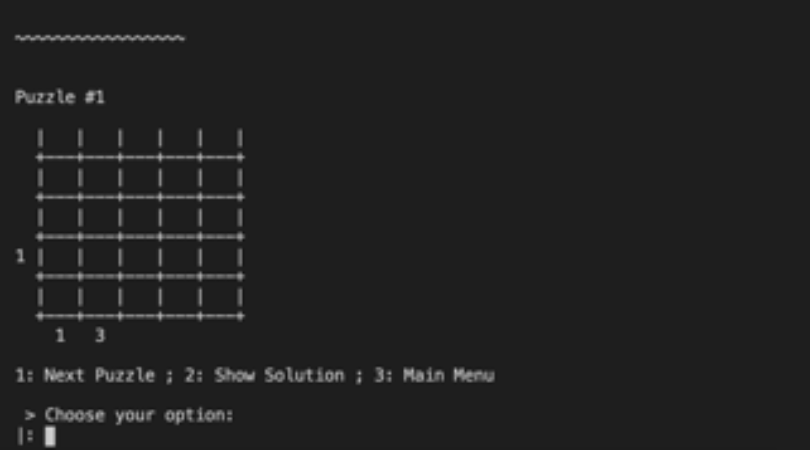
\includegraphics[scale=0.4]{img/3.png}
\end{center}

\paragraph{}
Aqui o utilizador pode escolher entre passar para o próximo puzzle (1), mostrar a solução do puzzle em questão (2) ou retornar para o menu principal.
Adicionalmente, o puzzle é sempre apresentado em branco.
 
\paragraph{}
Ao selecionar a primeira opção do menu anterior, o utilizador depara-se com o ecrã anterior. O puzzle 2 é resultado do predicado "show puzzle menu", contudo o número do puzzle passado como argumento é 2.

\paragraph{} 
Caso a segunda opção tenha sido escolhida, a solução do puzzle selecionado irá ser apresentada.

\begin{center}
    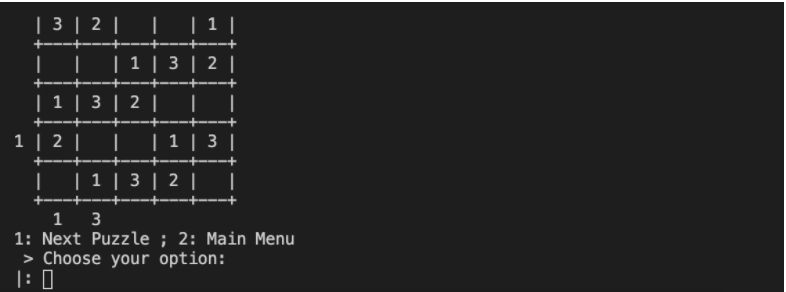
\includegraphics[scale=0.4]{img/4.png}
\end{center}

\paragraph{} 
Neste caso, o predicado "show solved puzzle menu" é chamado com o PuzzleNo igual a 2, que por sua vez, por meio da função starrynight, o predicado "display solution" é inicializado. Este último é responsável pelo preenchimento do puzzle com a solução encontrada.

\paragraph{} 
De volta ao menu principal, quando a segunda opção é selecionada, o utilizador consegue criar o seu próprio puzzle. O predicado "make your own menu" apresenta o seguinte menu:

\begin{center}
    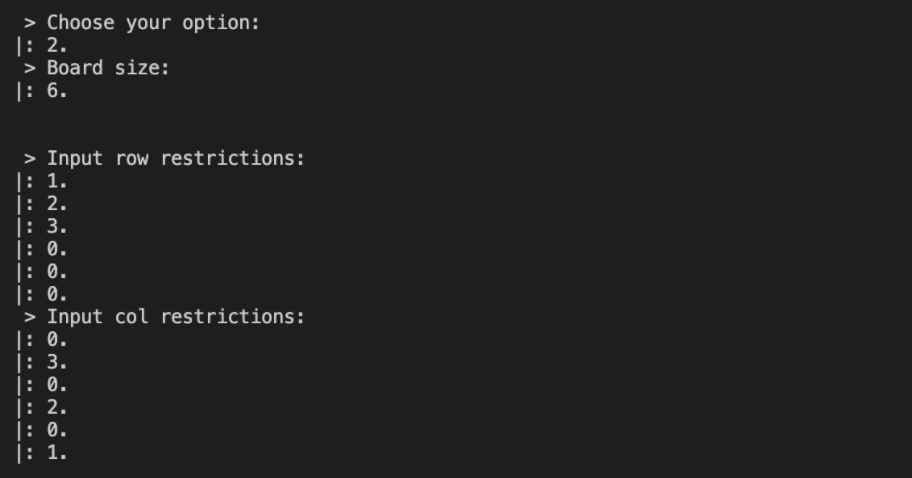
\includegraphics[scale=0.4]{img/5.png}
\end{center}

\paragraph{} 
Por motivos de demonstração, apenas se irá considerar um puzzle 6x6. As restrições deste novo tabuleiro são introduzidas no sentido última para primeira. Ou seja, a primeira restrição introduzida (‘row restriction -> 1.’) é a que vai ser aplicada no canto inferior esquerdo (primeira row). As colunas e as suas restrições se comportam de forma análoga. 

\paragraph{} 
Finalmente, a solução é mostrada da seguinte forma:

\begin{center}
    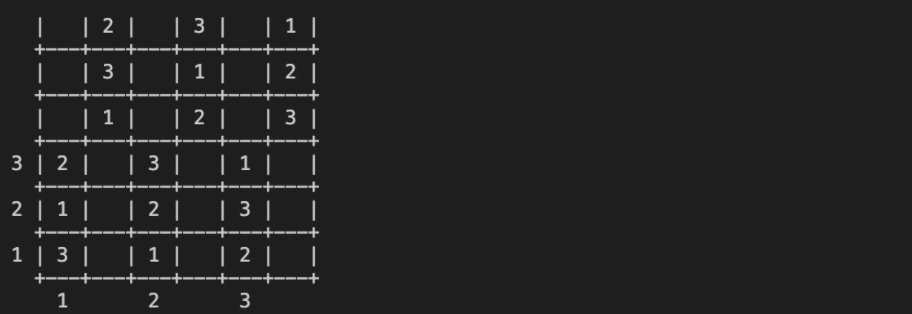
\includegraphics[scale=0.4]{img/6.png}
\end{center}

\paragraph{} 
Esta solução é demonstrada utilizando, mais uma vez, o predicado "display solution".

%%%%%%%%%%%%%%%%%%%%%%%%%%
\section{Resultados}

\begin{center}
    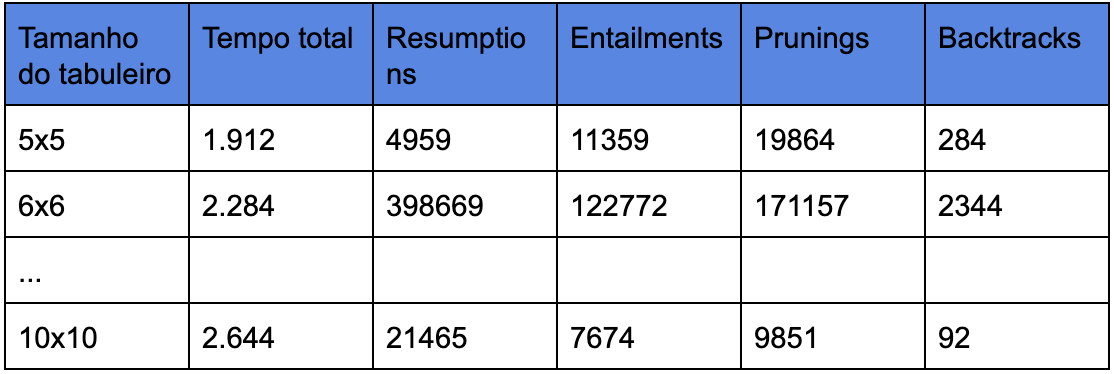
\includegraphics[scale=0.4]{img/7.png}
\end{center}

\paragraph{}
O problema não apresenta solução para tabuleiros de dimensão inferior a 5x5 devido às restrições impostas. Tabuleiros dessa dimensão ou não permitem a inclusão dos 3 símbolos numa linha / coluna (caso do tabuleiro 2x2), ou não permitem a não repetição do símbolo na diagonal adjacente.
Para tabuleiros de dimensão superior a 10x10, a performance do código apresenta menor eficiência. 
A fiabilidade dos resultados apresentados na tabela anterior, encontra-se comprometida pela reduzida dimensão da amostra (4 puzzles para cada dimensão), dado que não foi implementado um gerador de puzzles.

%%%%%%%%%%%%%%%%%%%%%%%%%%
\section{Conclusões e Trabalho Futuro}

\paragraph{}
O trabalho teve como objectivo implementar um programa com capacidade para atingir uma solução para qualquer variação do puzzle Starry Night, através da aplicação dos conceitos relativos à Programação em Lógica com restrições.
O trabalho desenvolvido encontra solução para tabuleiros de dimensão igual ou superior a 5x5 e demonstra-se eficiente para tabuleiros de dimensões até 10x10. Para tabuleiros de dimensão superior a 10x10, a eficiência fica comprometida, dado que o processo para atingir uma solução possível torna-se muito lento.
Referimos por último que, em toda a extensão deste artigo, quando mencionada a eficiência da aplicação, foi considerado que o utilizador impõe sempre um número razoável de restrições. Tendo em consideração o elevado número possibilidades de escolha, em termos de número de restrições flexíveis que o utilizador tem, a sua contabilização torna-se impraticável.

%%%%%%%%%%%%%%%%%%%%%%%%%%
\section{Bibiografia}

\paragraph{}
Para a realização deste trabalho foram apenas utilizados os slides disponibilizados da cadeira Programação em Lógica. 

%%%%%%%%%%%%%%%%%%%%%%%%%%
\section{Anexo}

\subsection{starynight.pl}
\begin{center}
    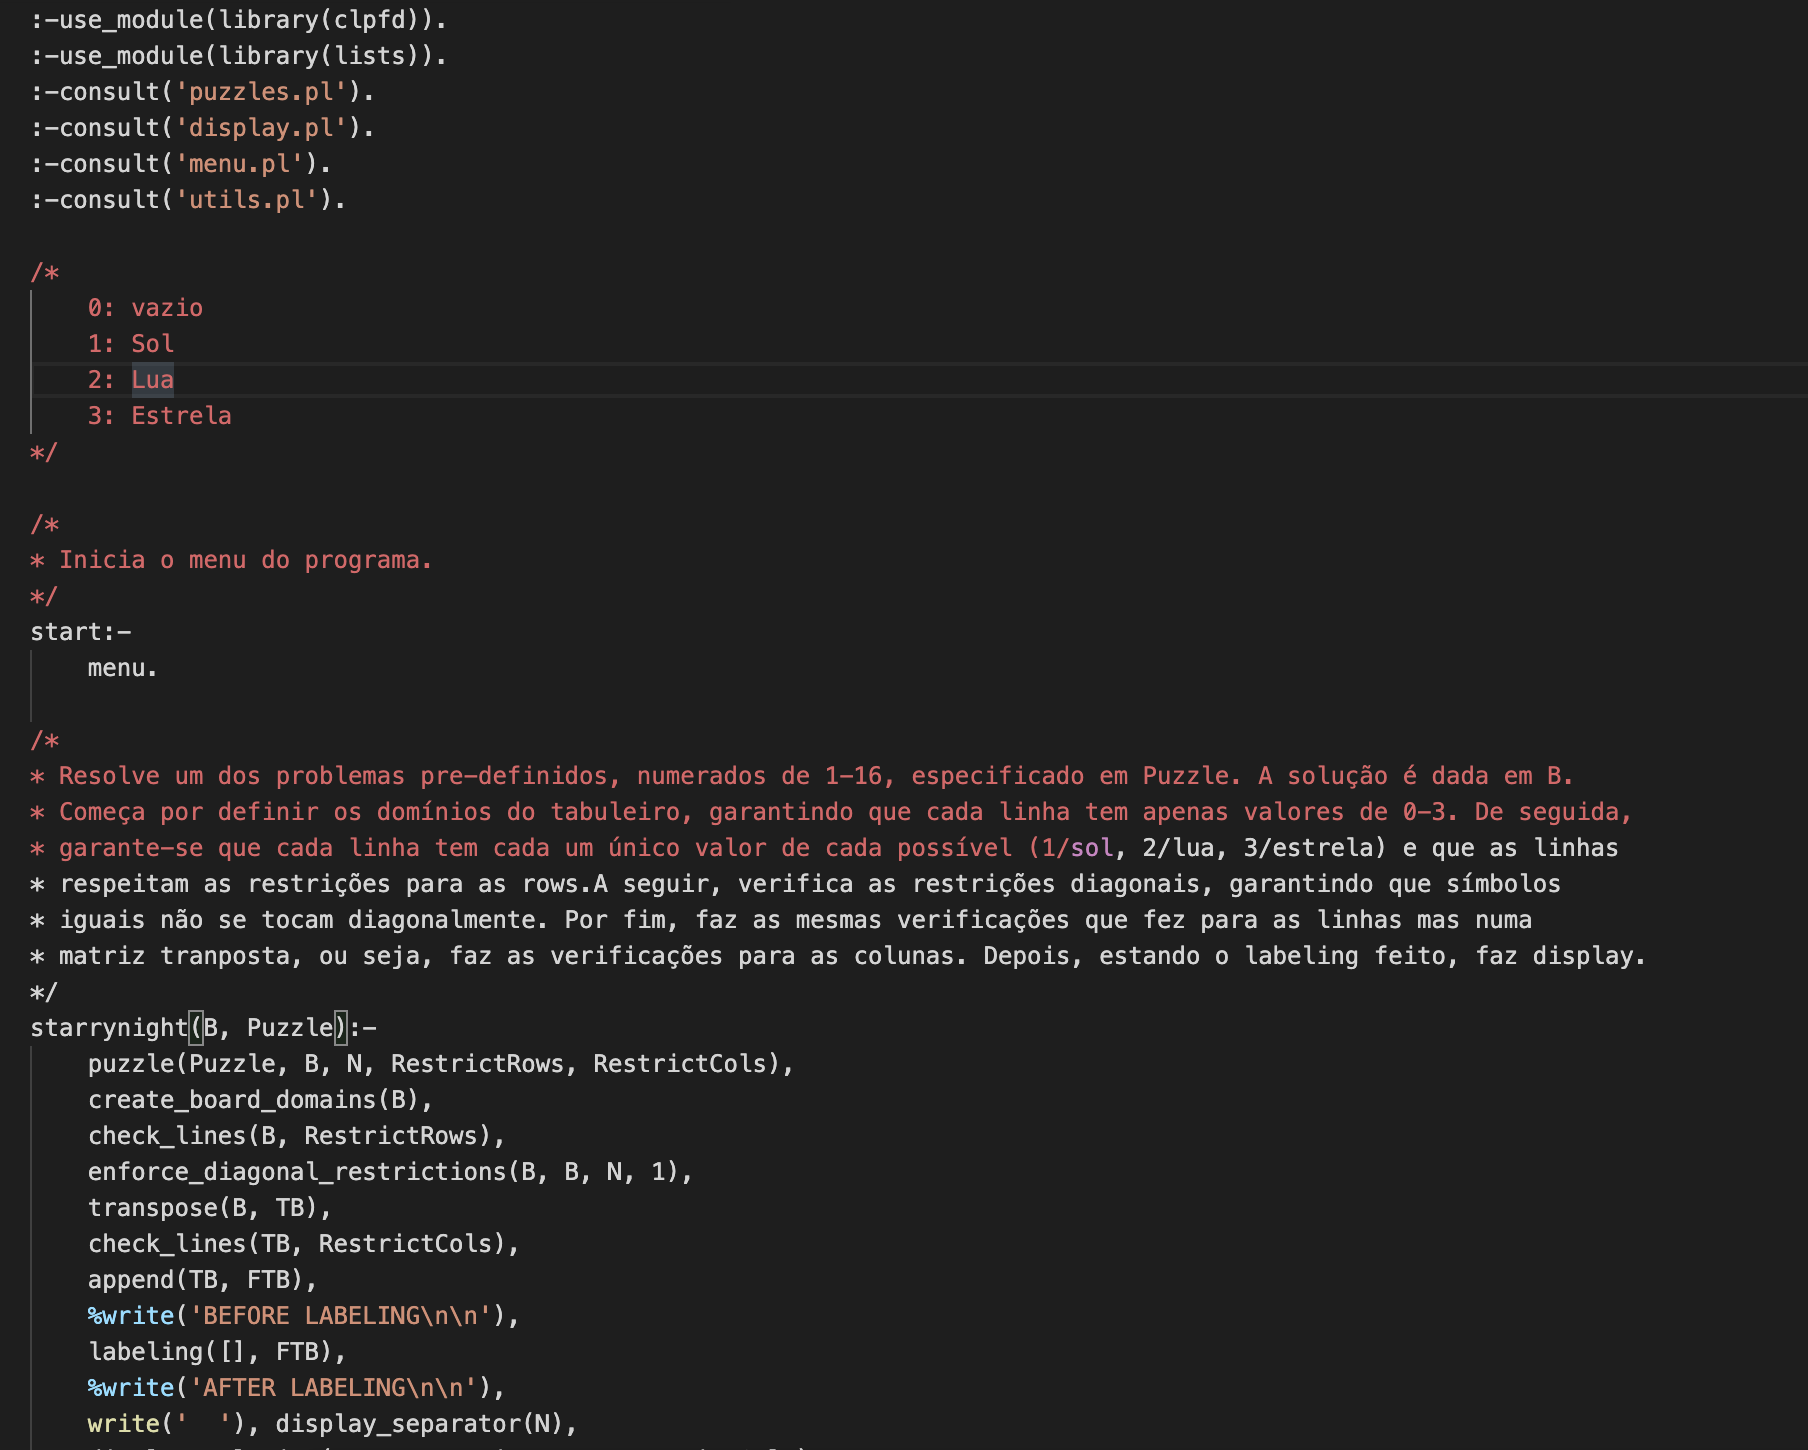
\includegraphics[scale=0.4]{img/8.png}
    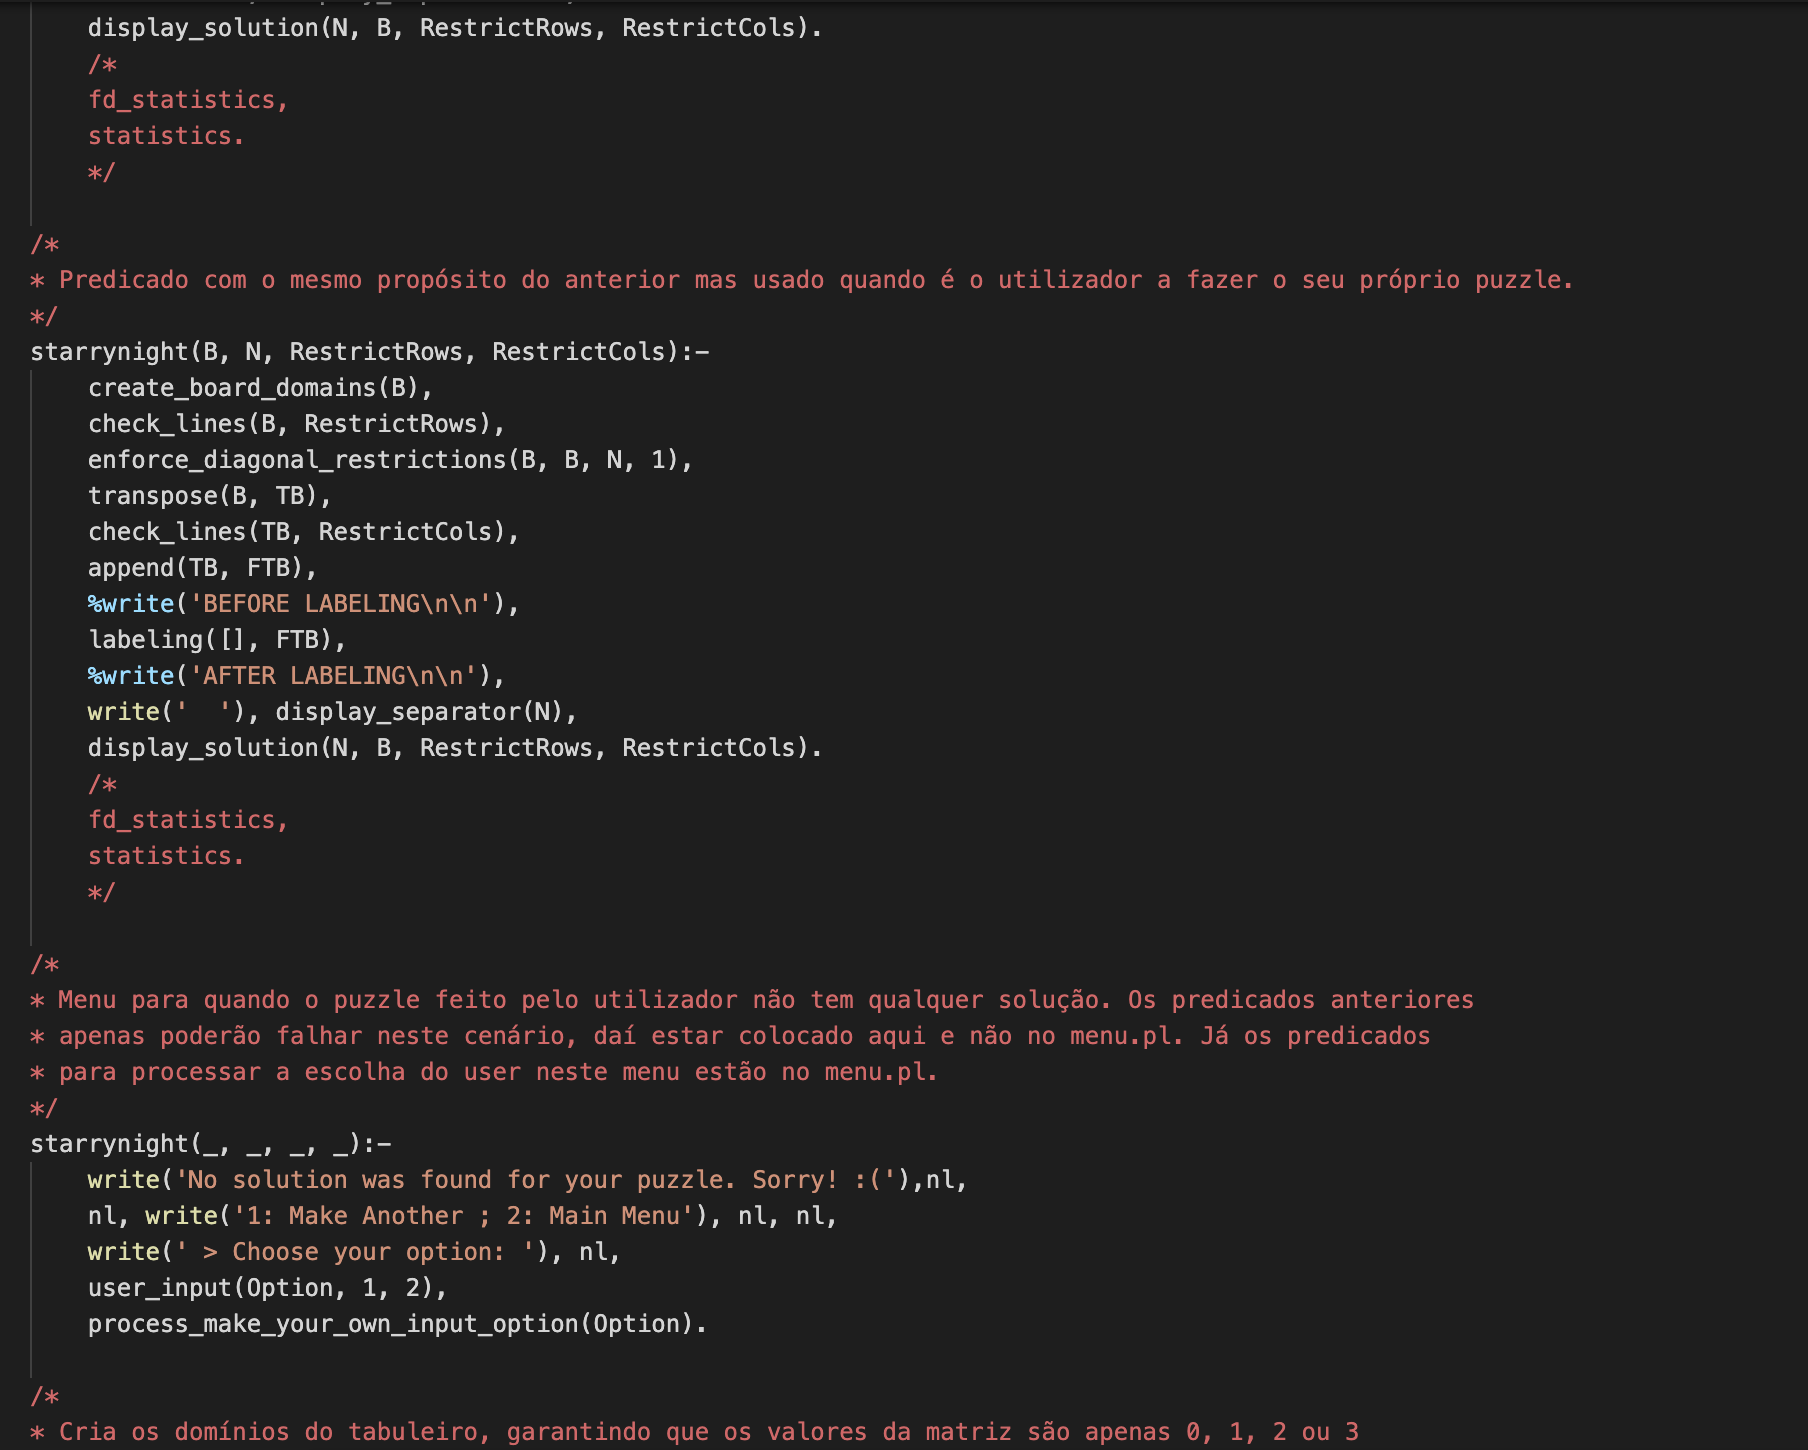
\includegraphics[scale=0.4]{img/9.png}
    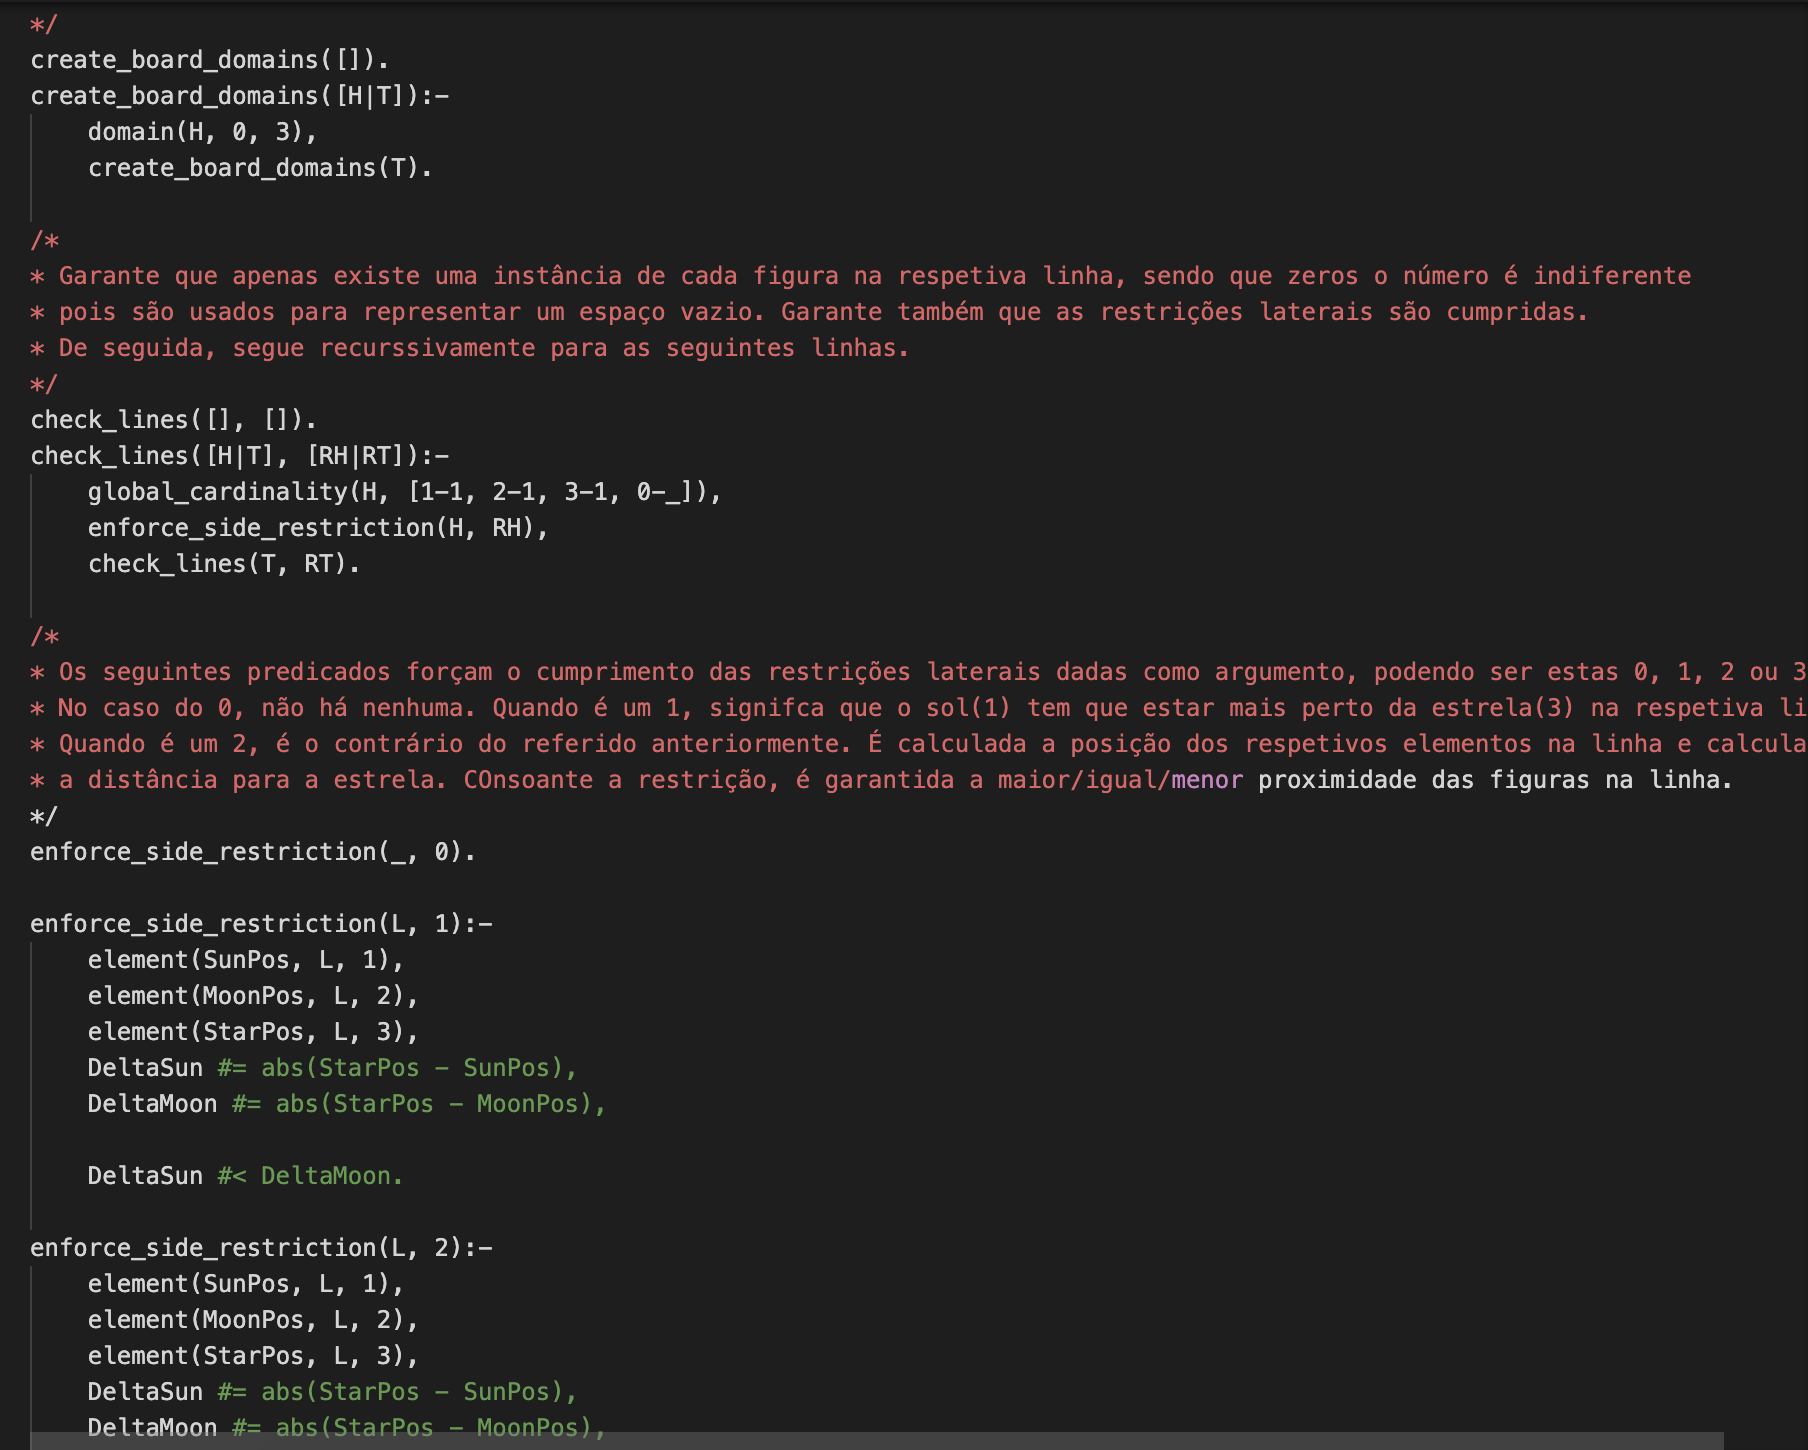
\includegraphics[scale=0.4]{img/10.png}
    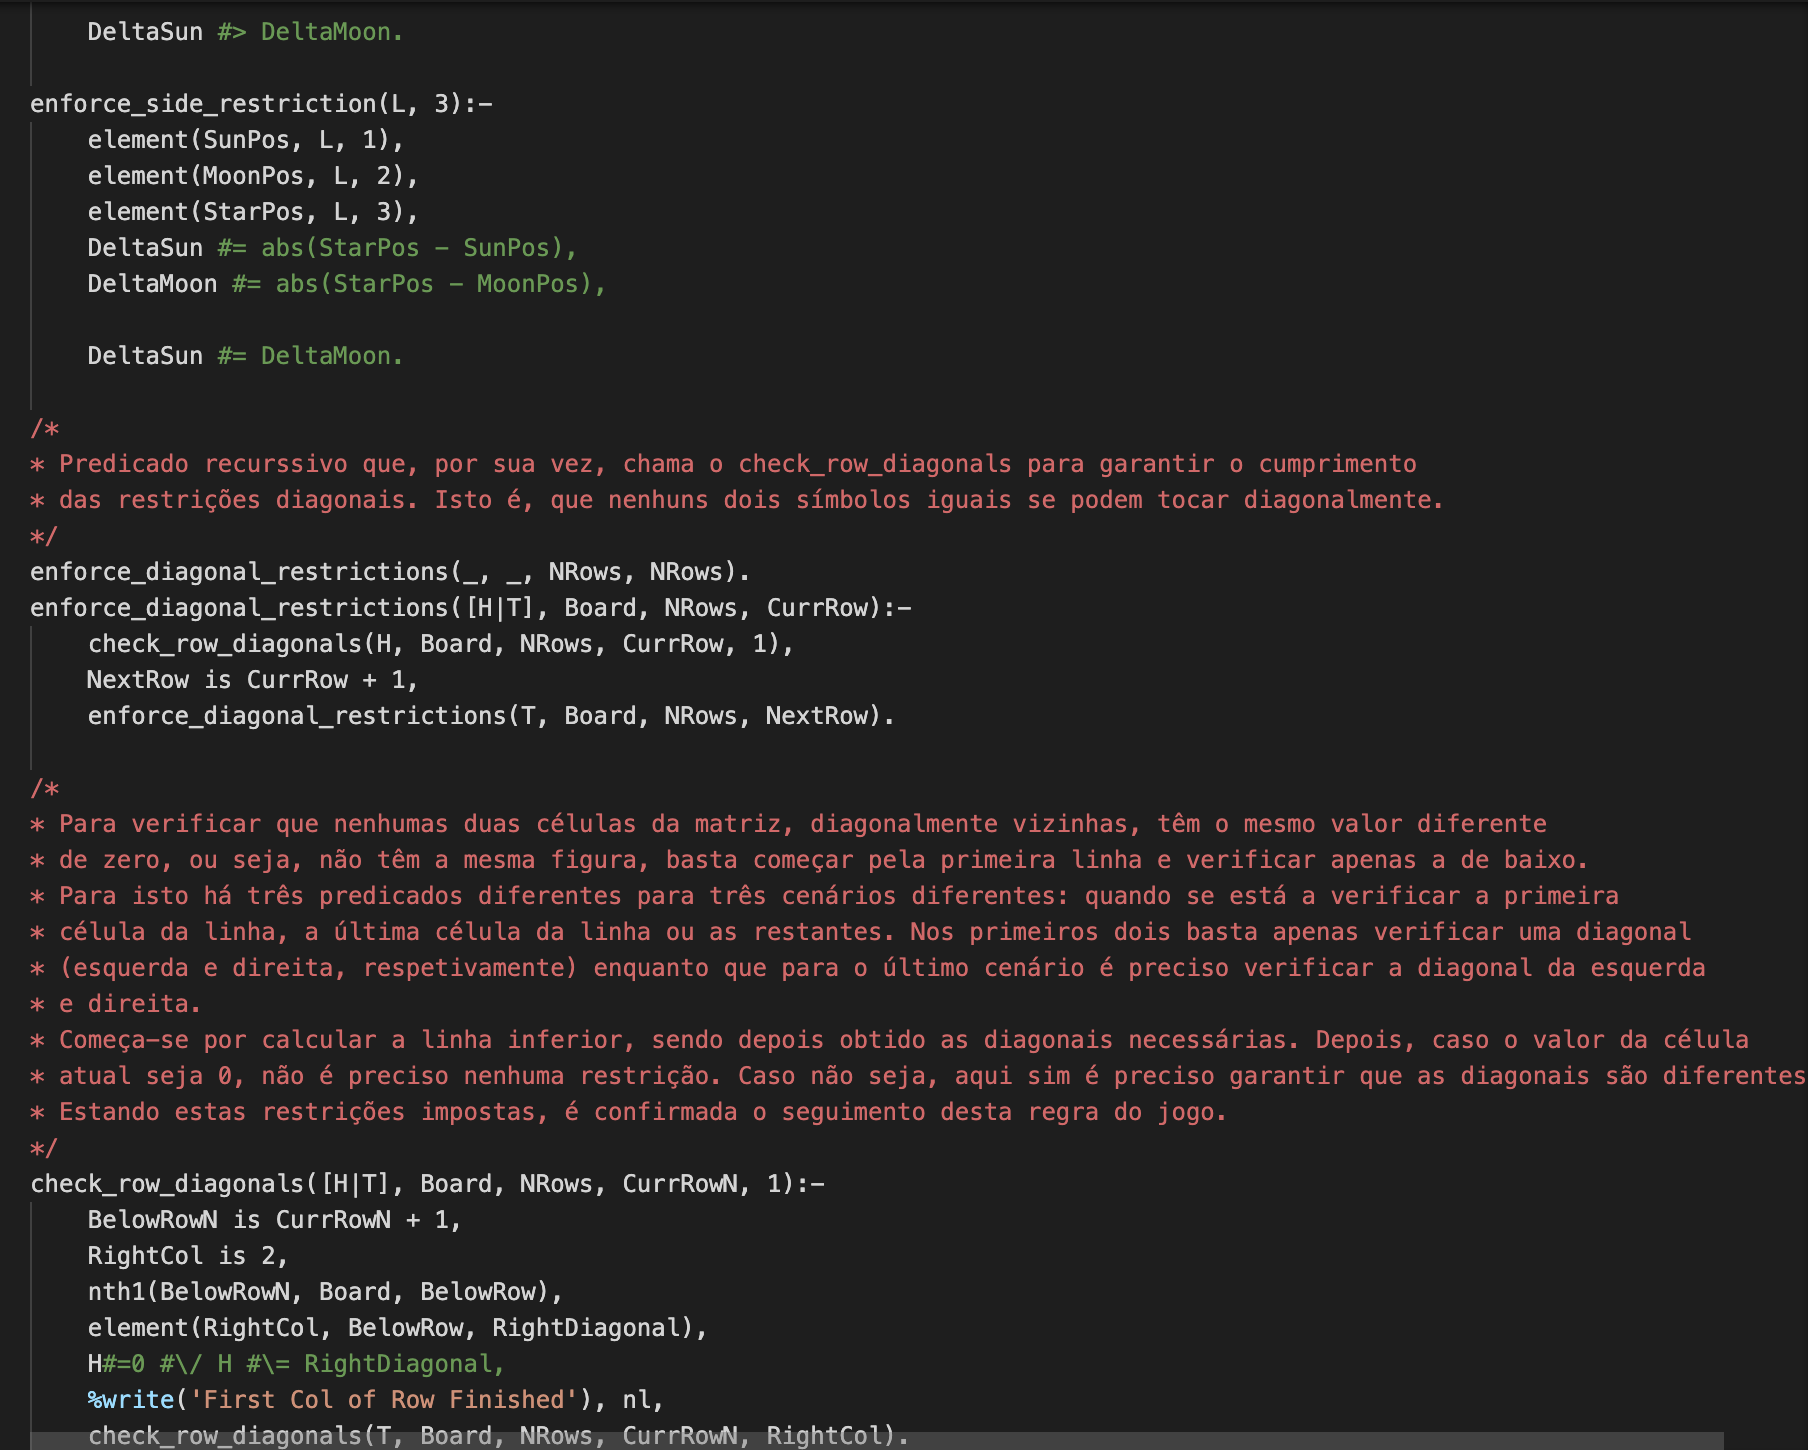
\includegraphics[scale=0.4]{img/11.png}
    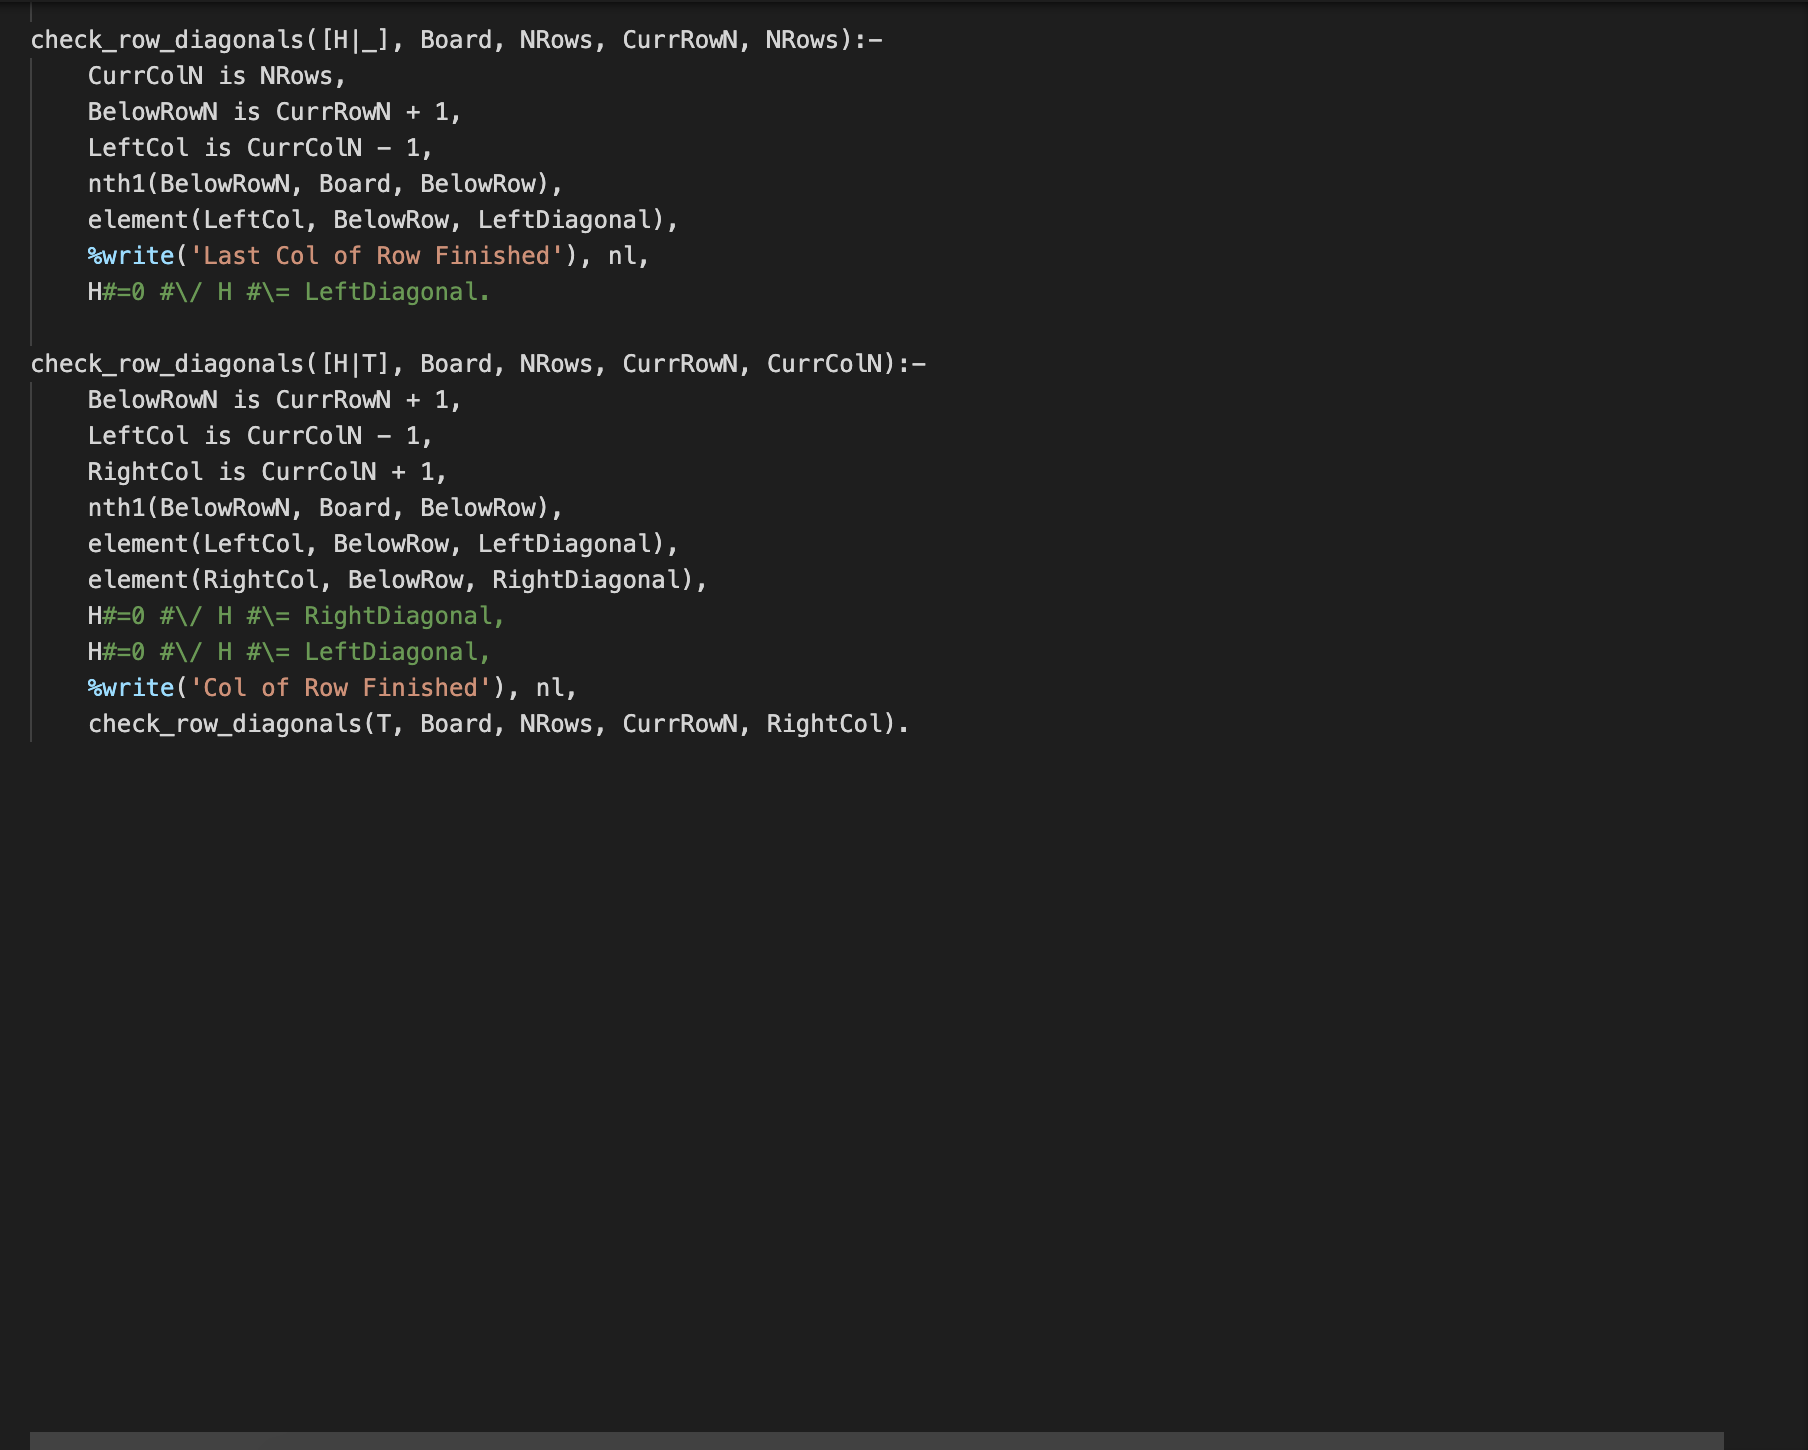
\includegraphics[scale=0.4]{img/12.png}
\end{center}

\subsection{menu.pl}
\begin{center}
    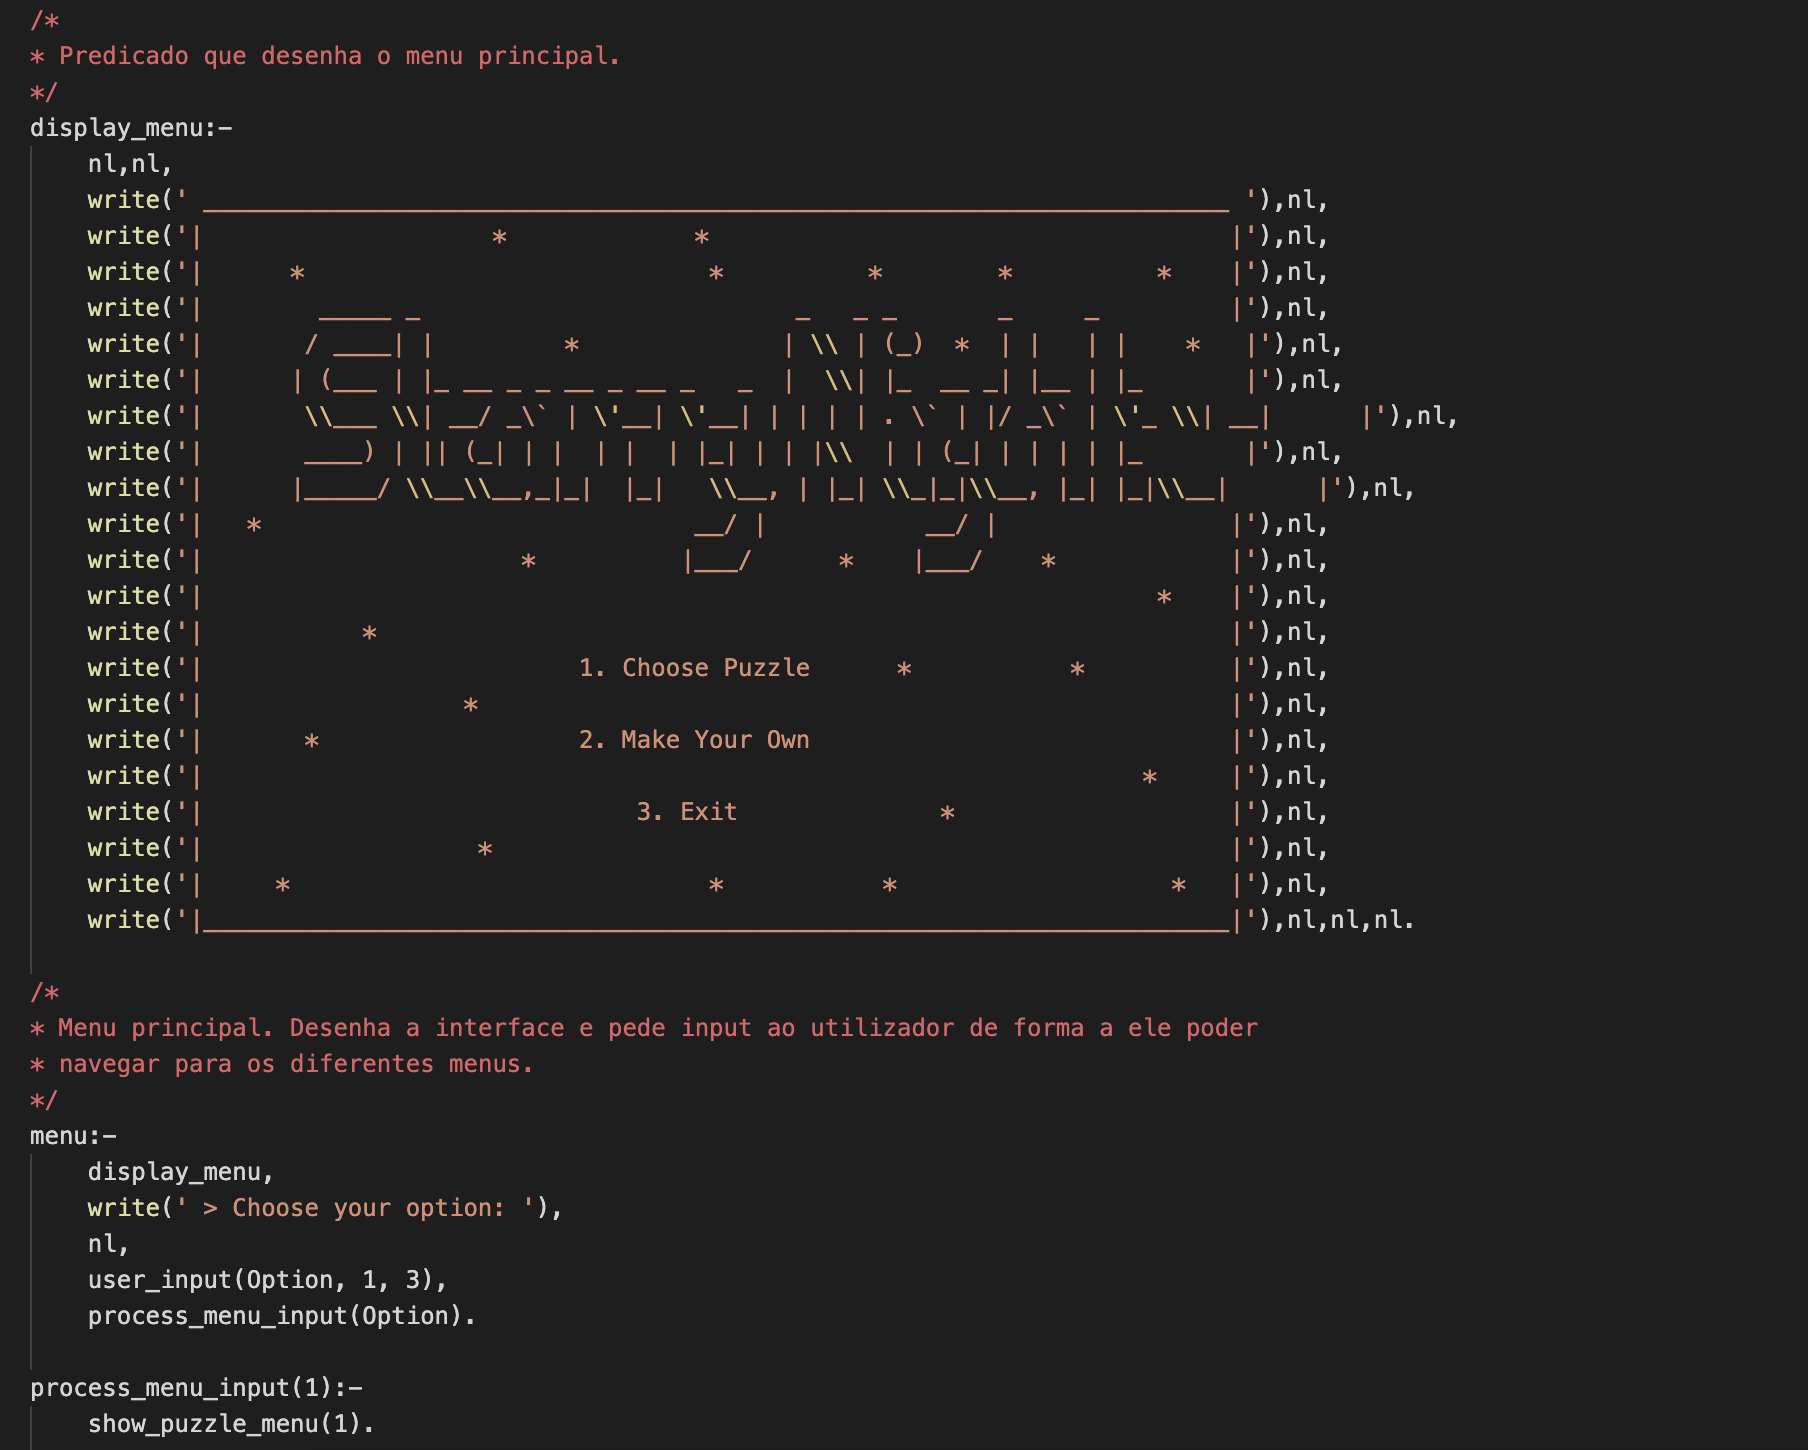
\includegraphics[scale=0.4]{img/13.png}
    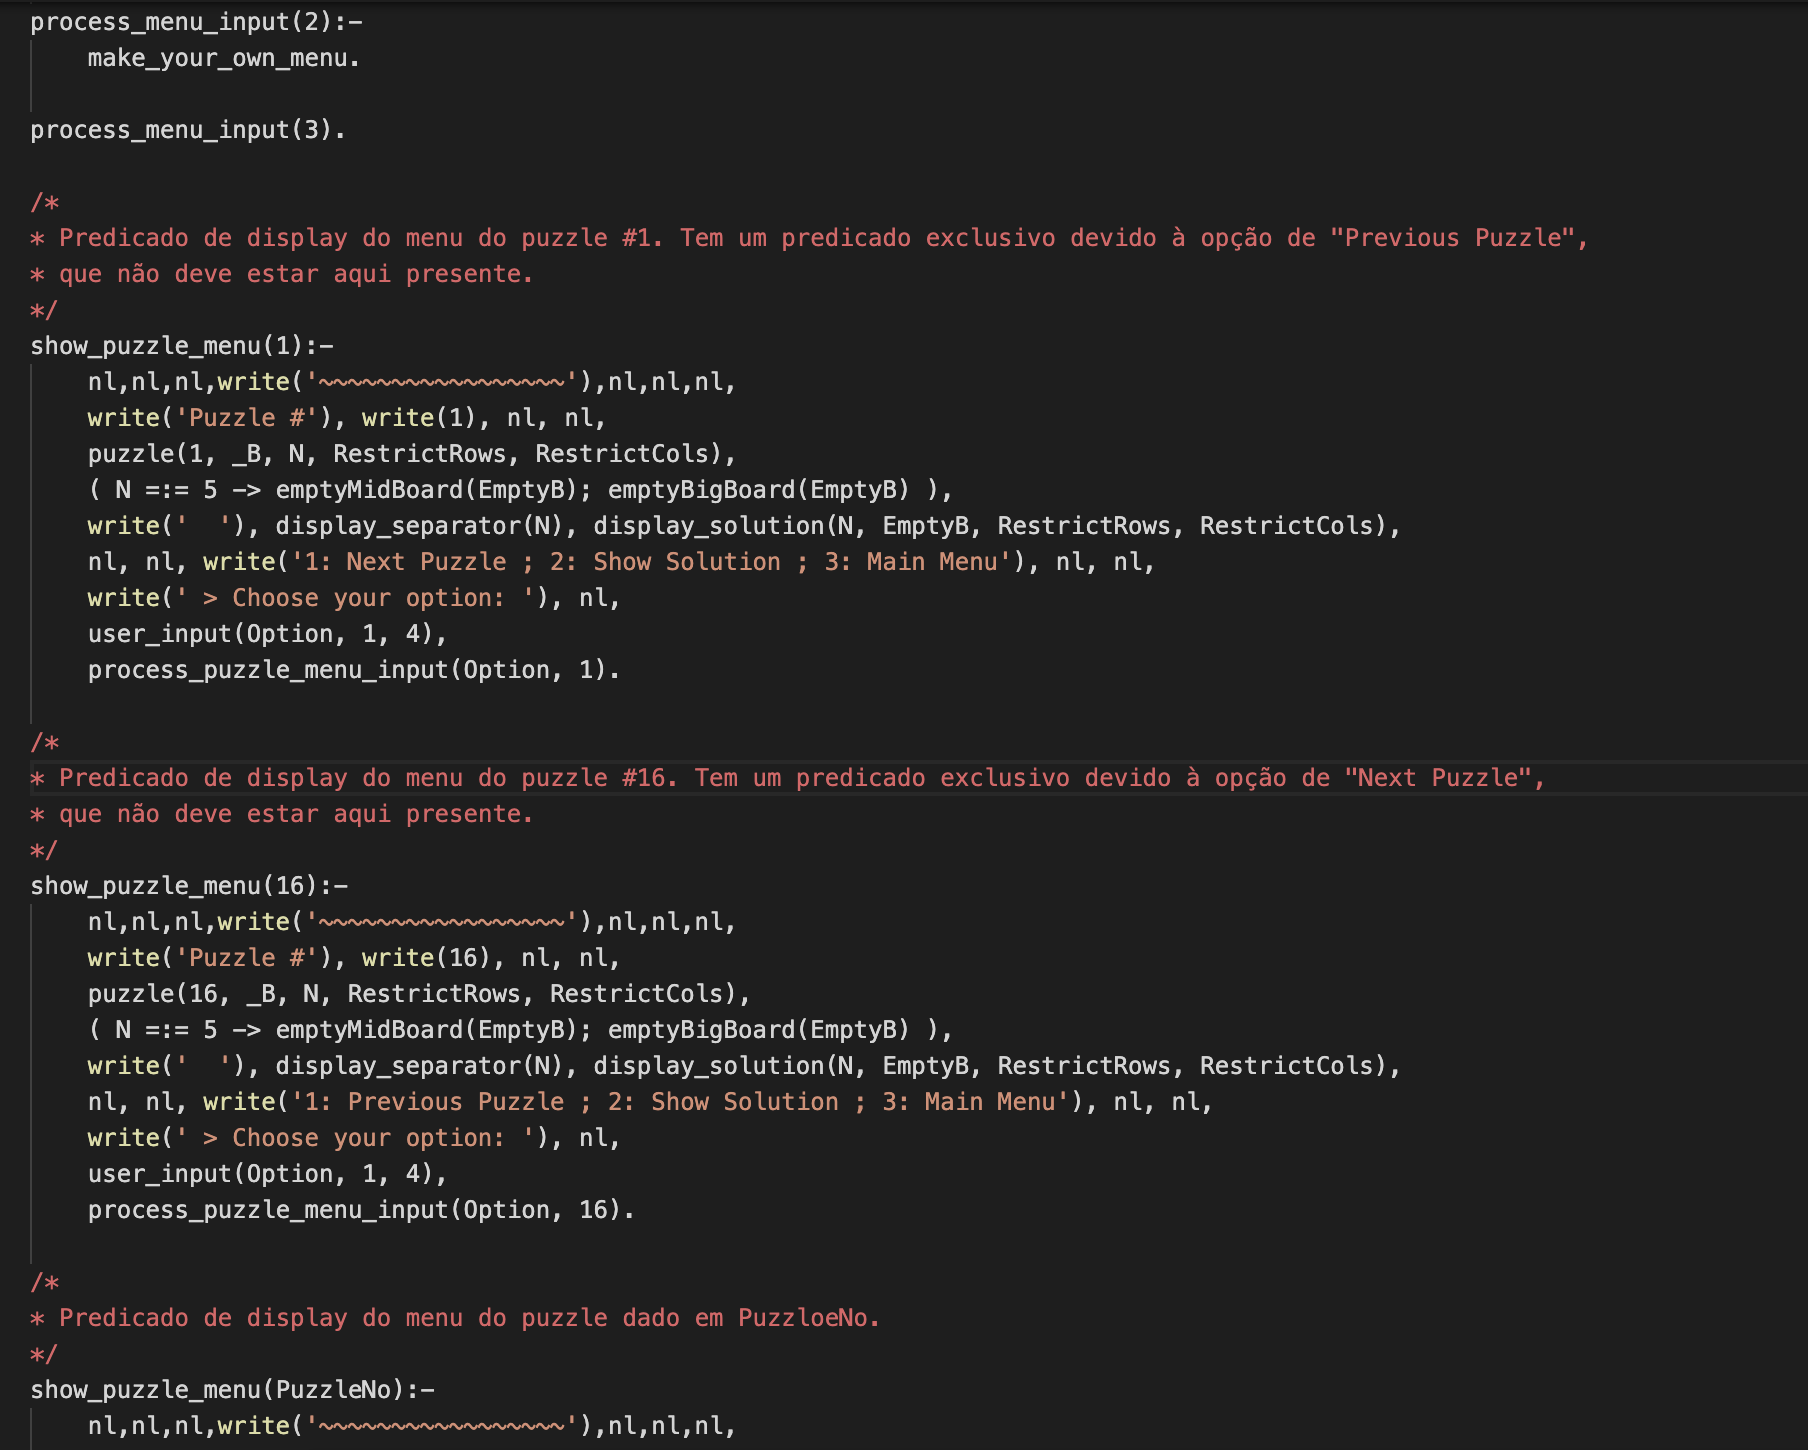
\includegraphics[scale=0.4]{img/14.png}
    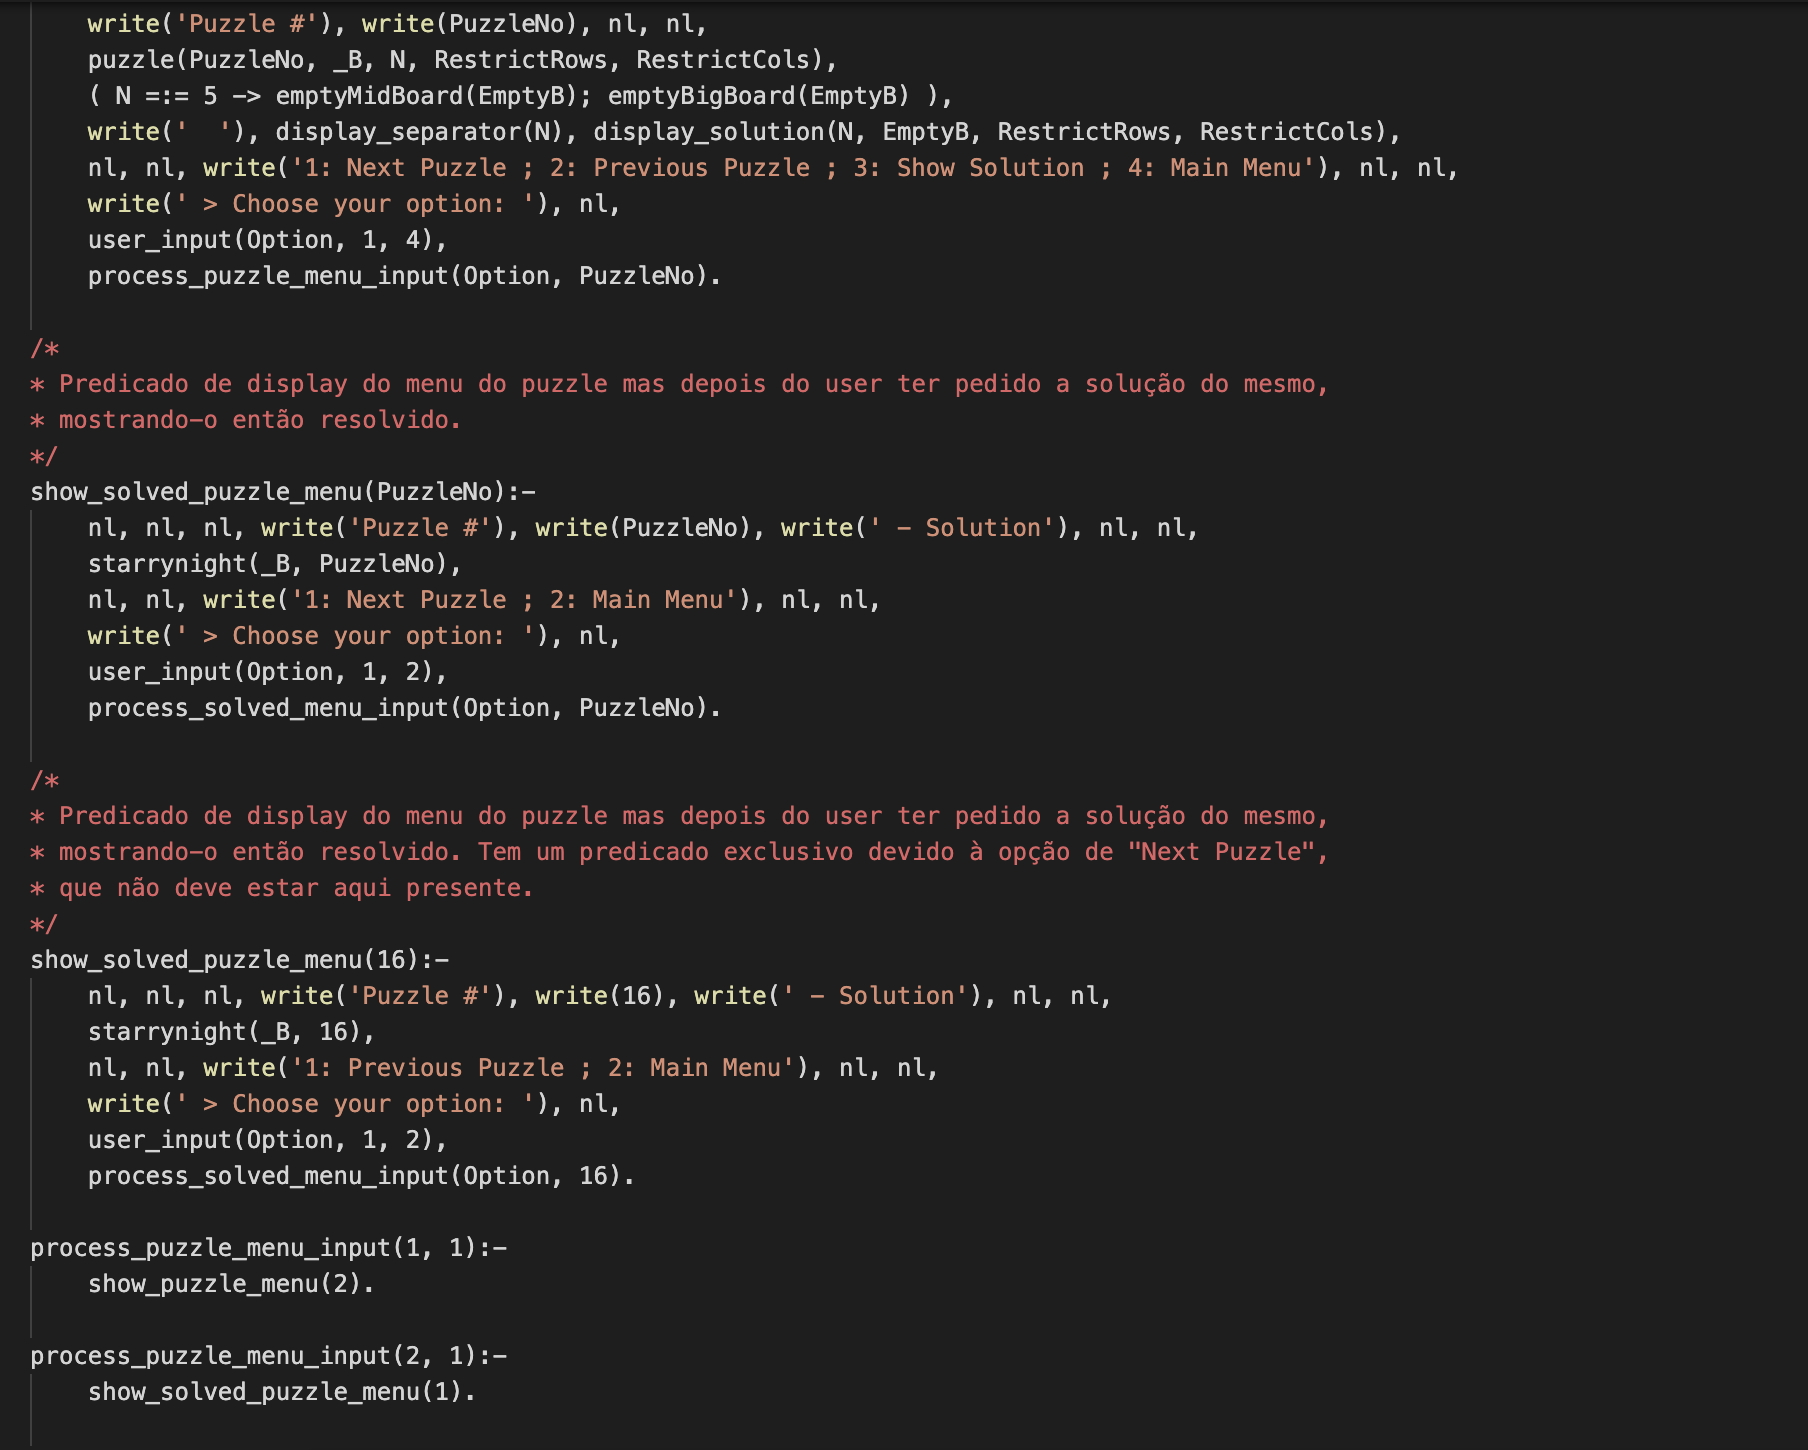
\includegraphics[scale=0.4]{img/15.png}
    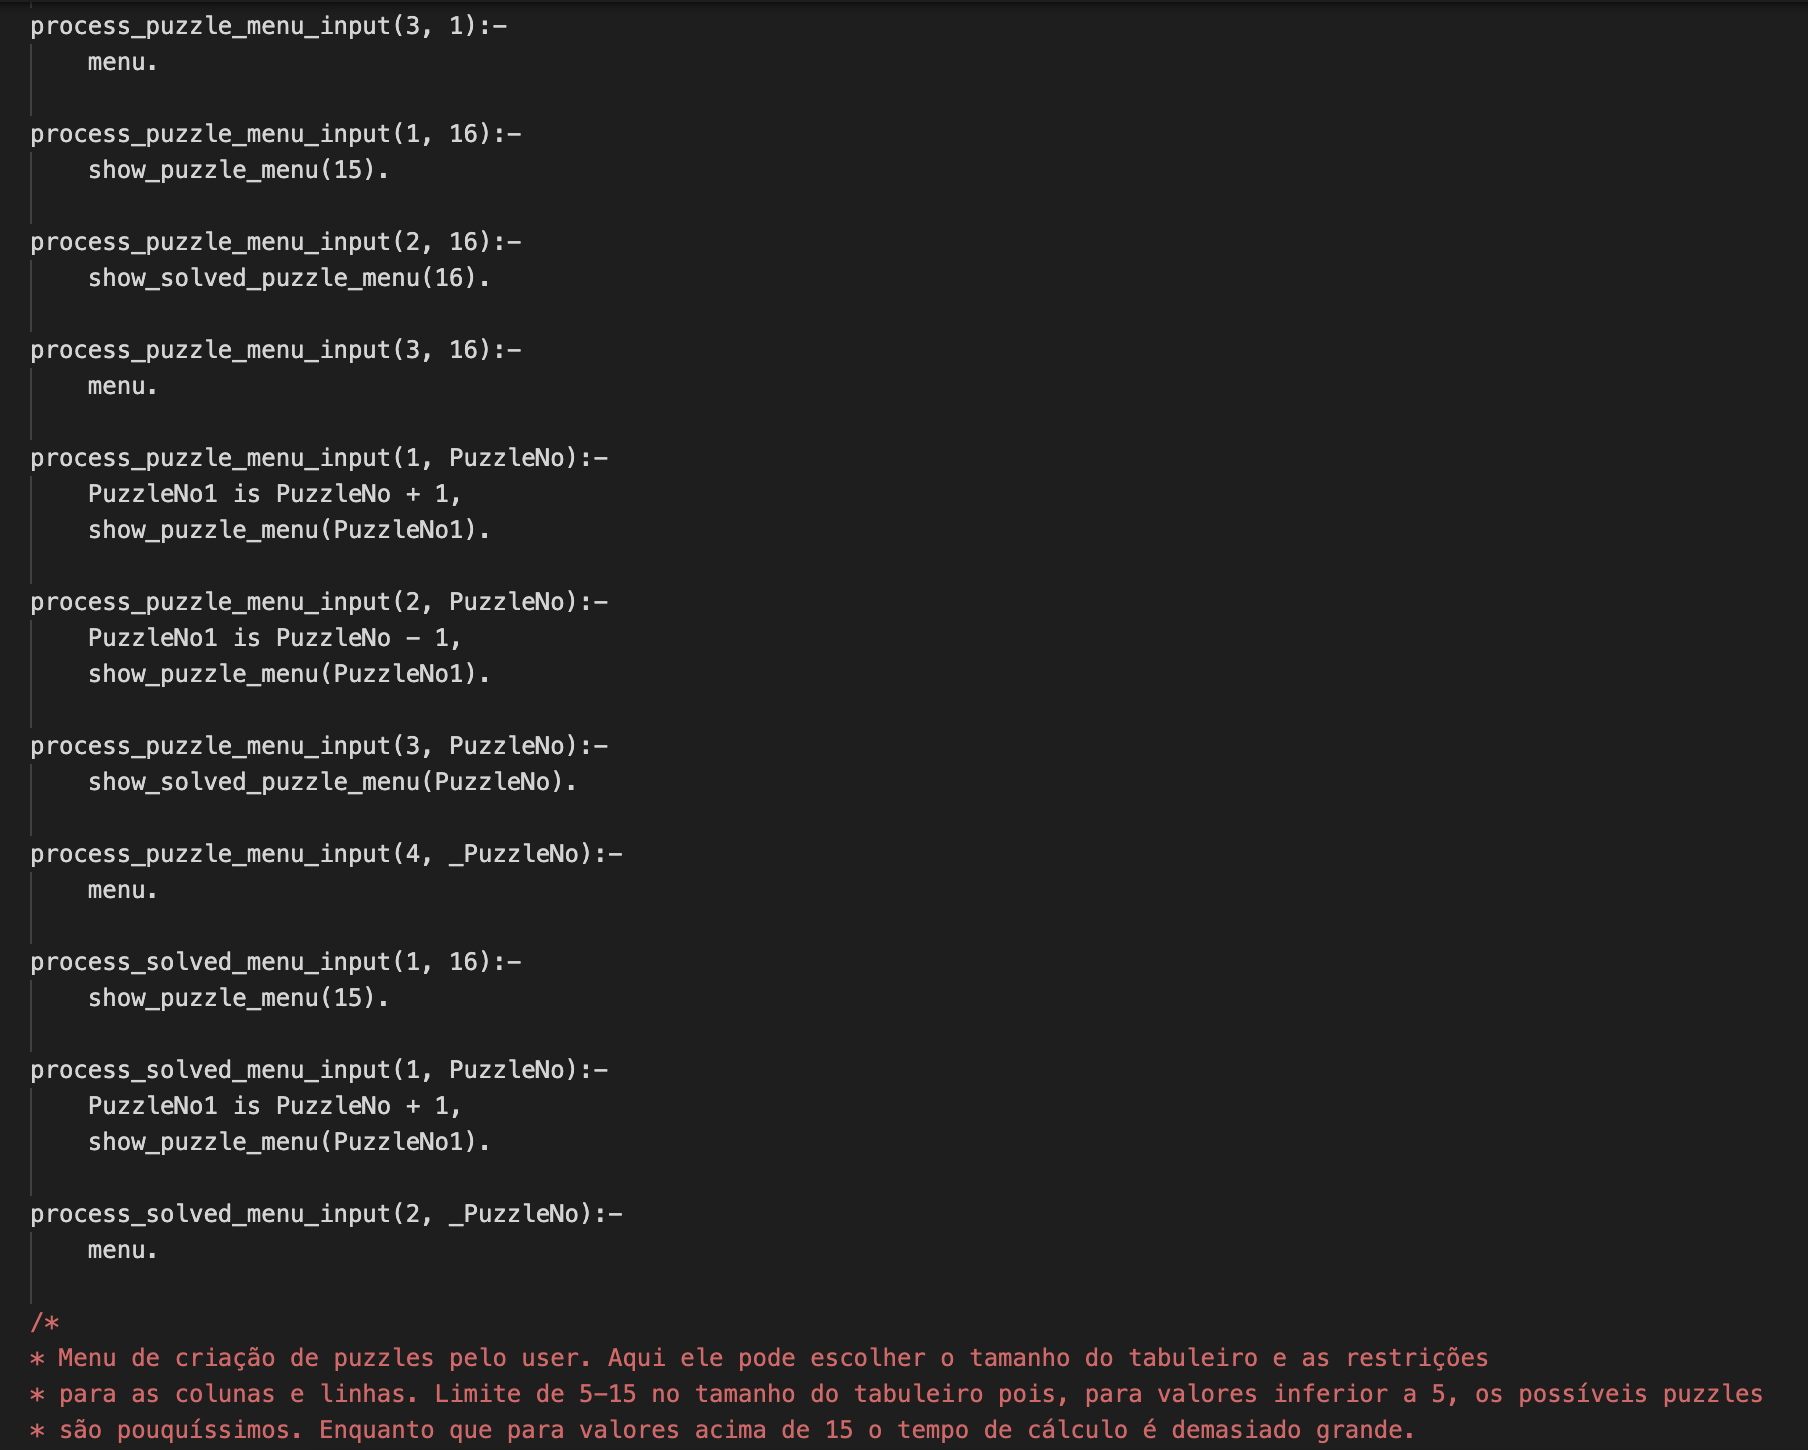
\includegraphics[scale=0.4]{img/16.png}
    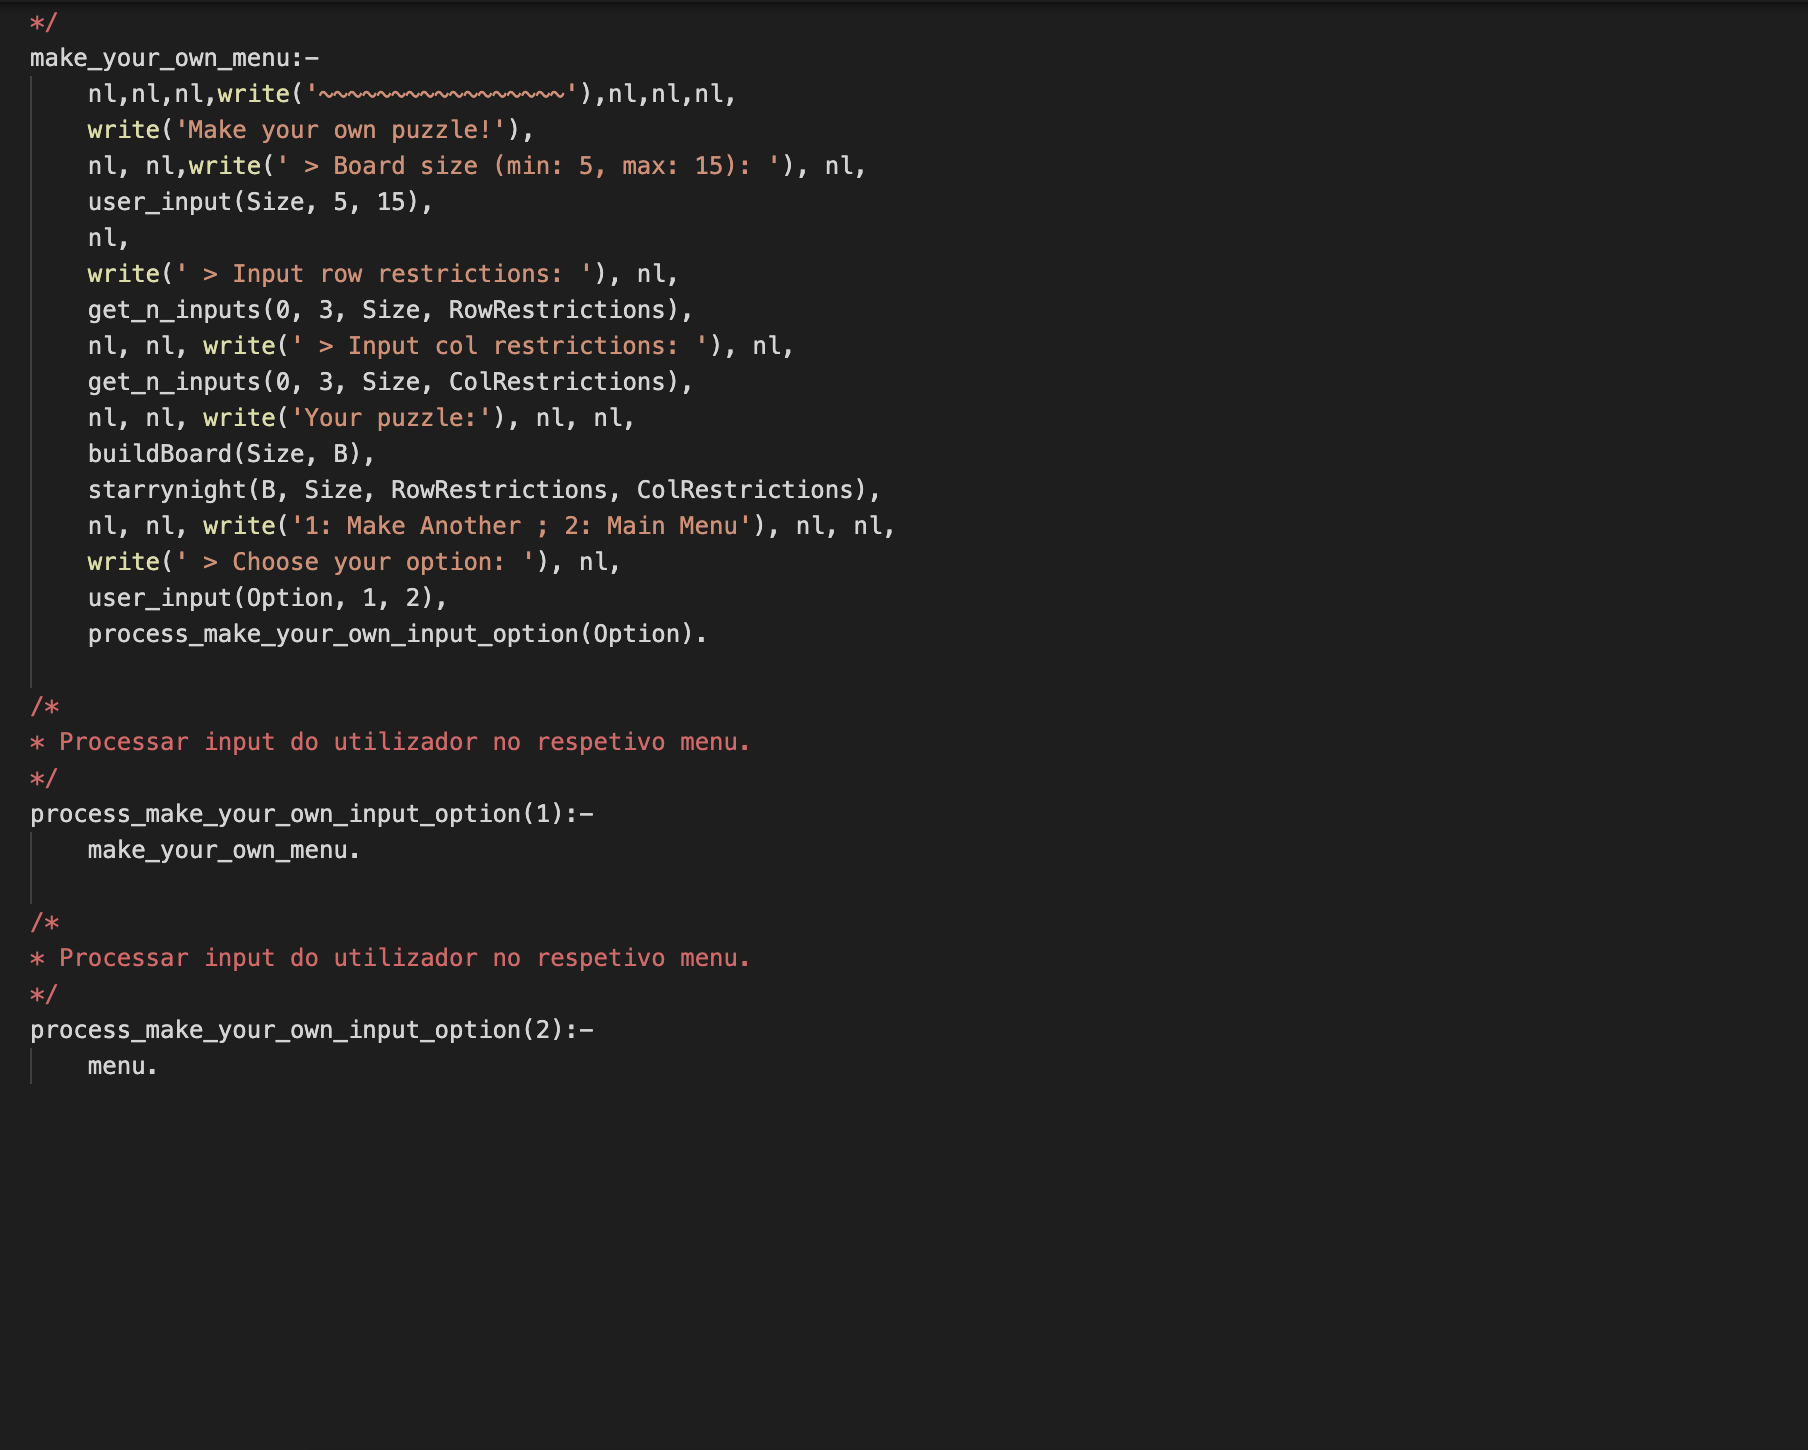
\includegraphics[scale=0.4]{img/17.png}
\end{center}

\subsection{puzzles.pl}
\begin{center}
    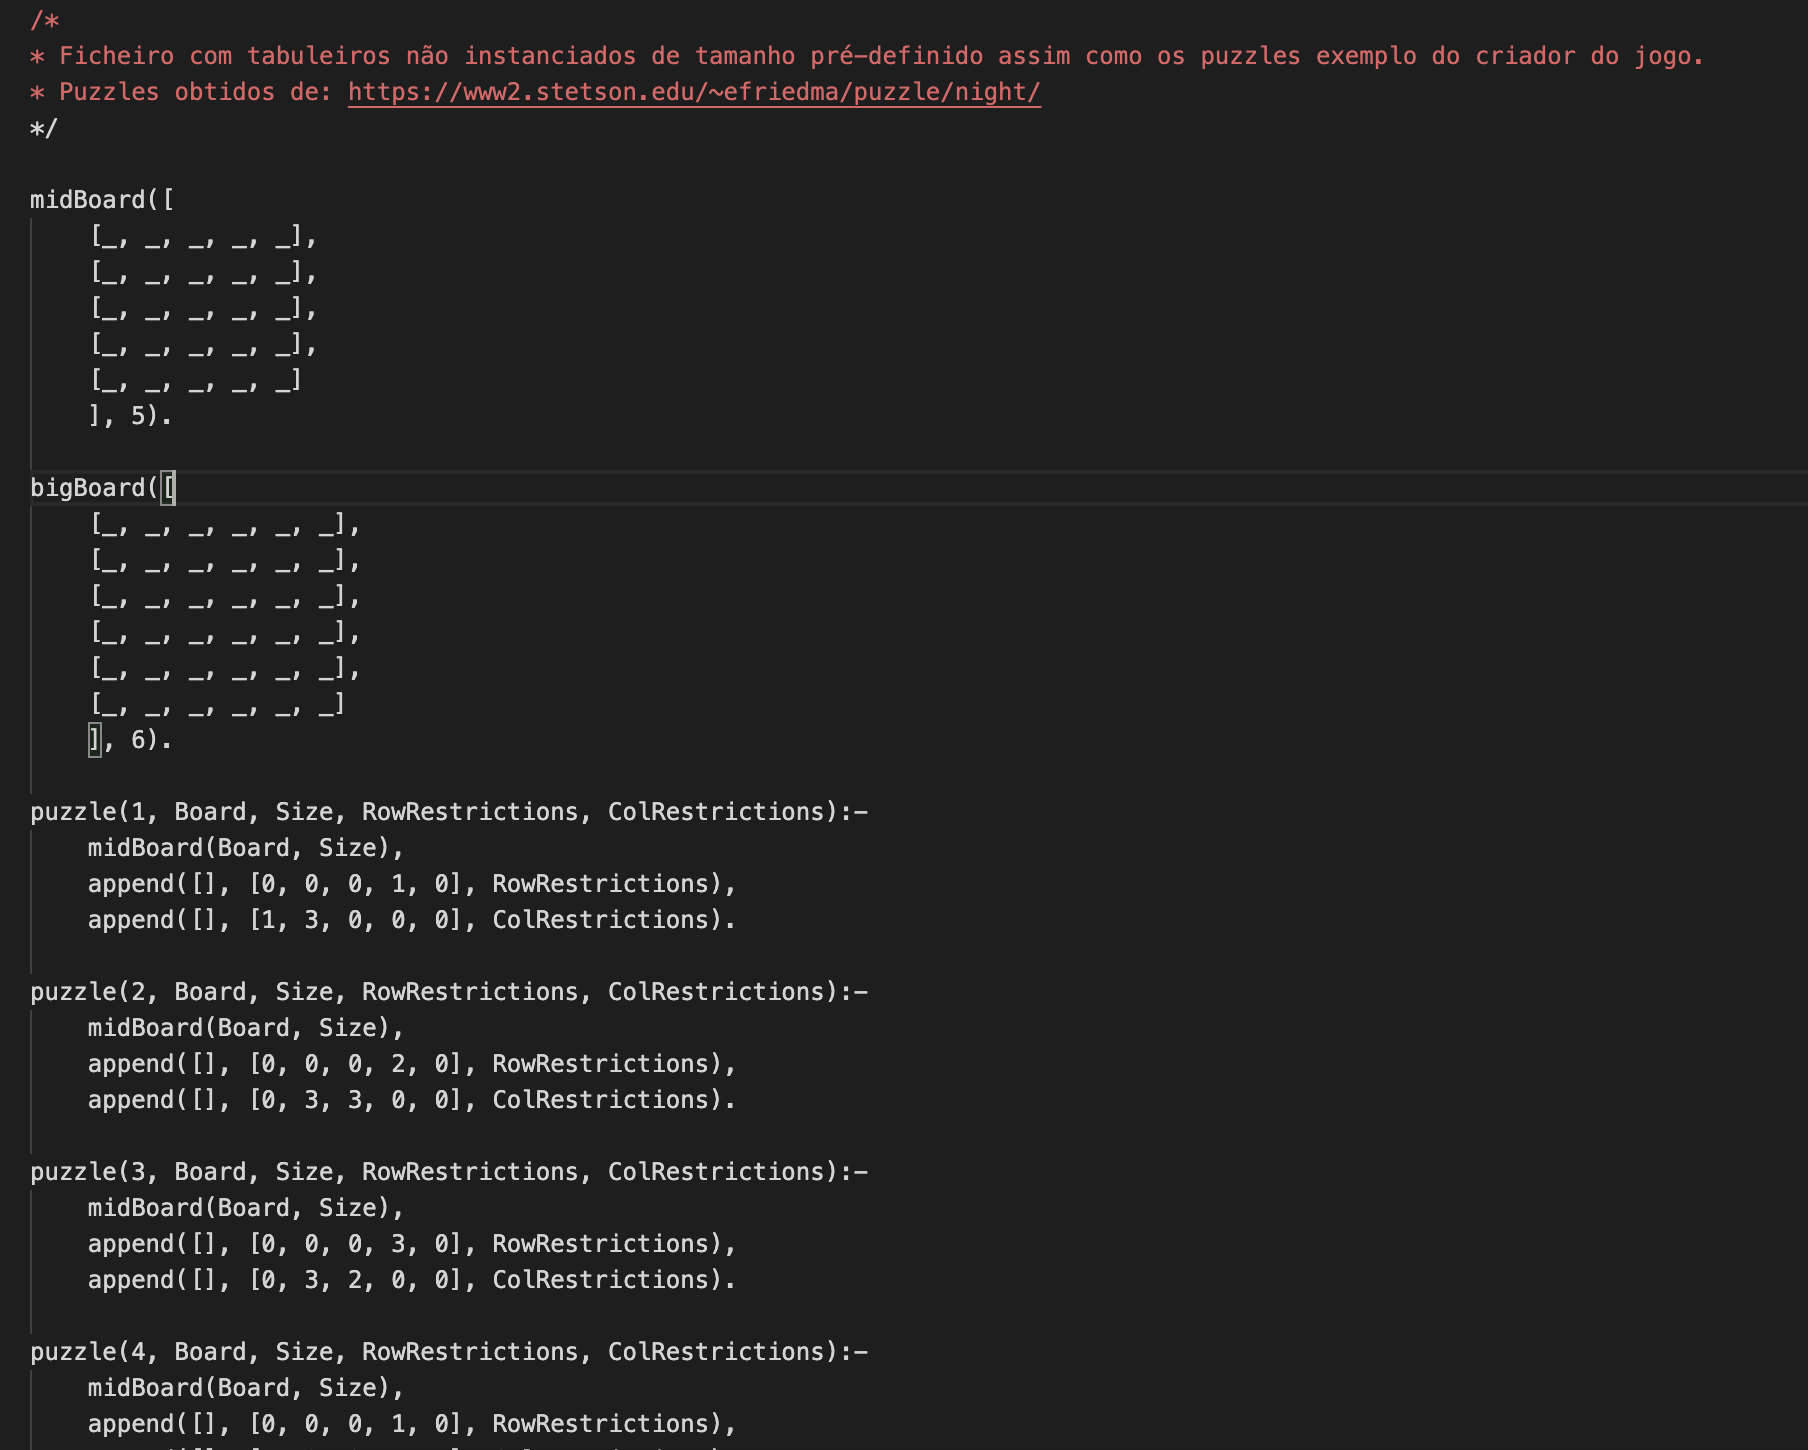
\includegraphics[scale=0.4]{img/18.png}
    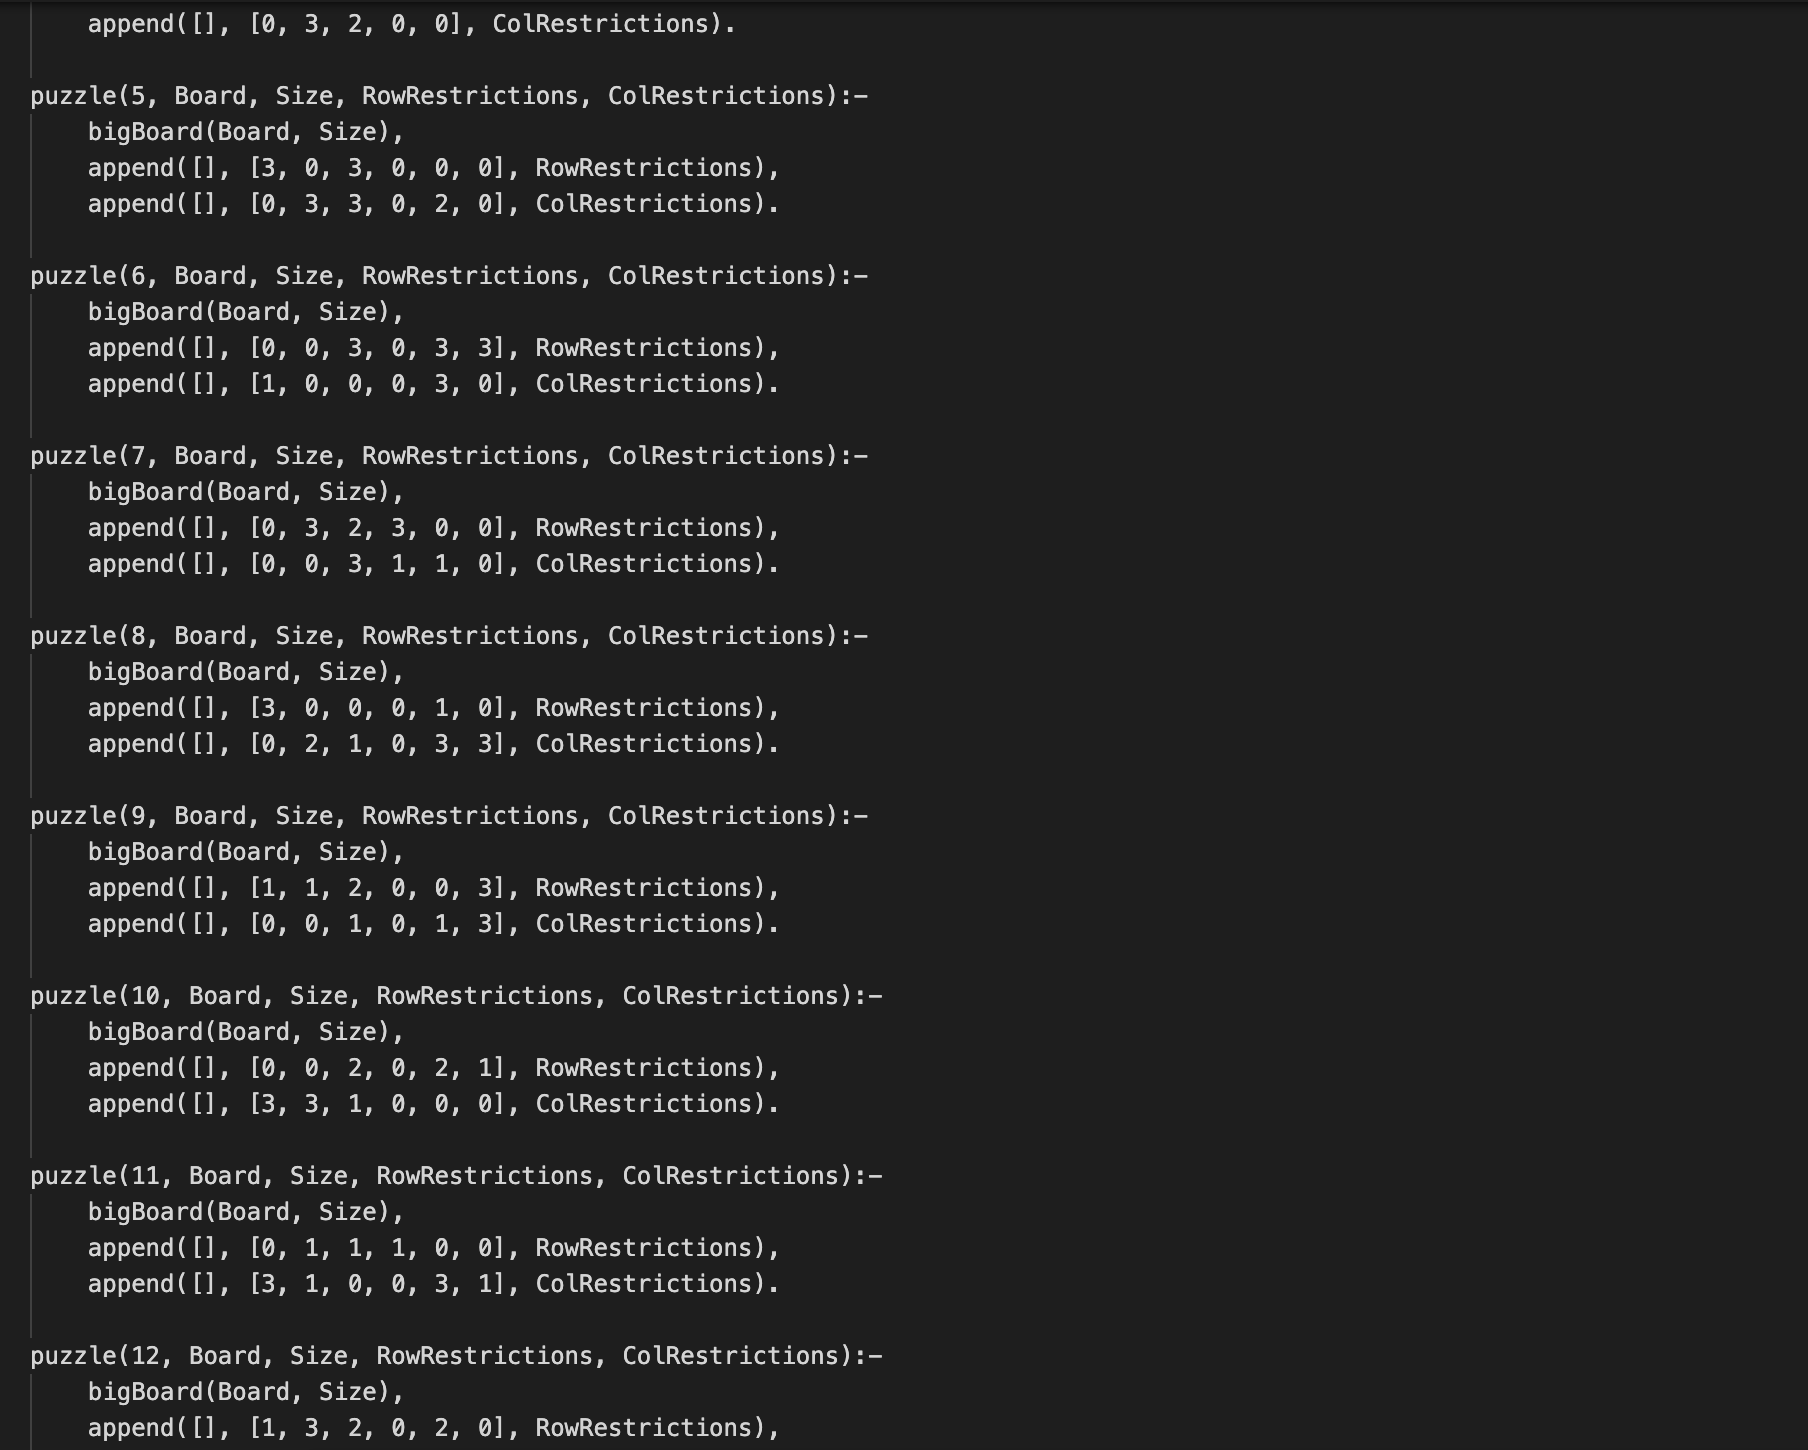
\includegraphics[scale=0.4]{img/19.png}
    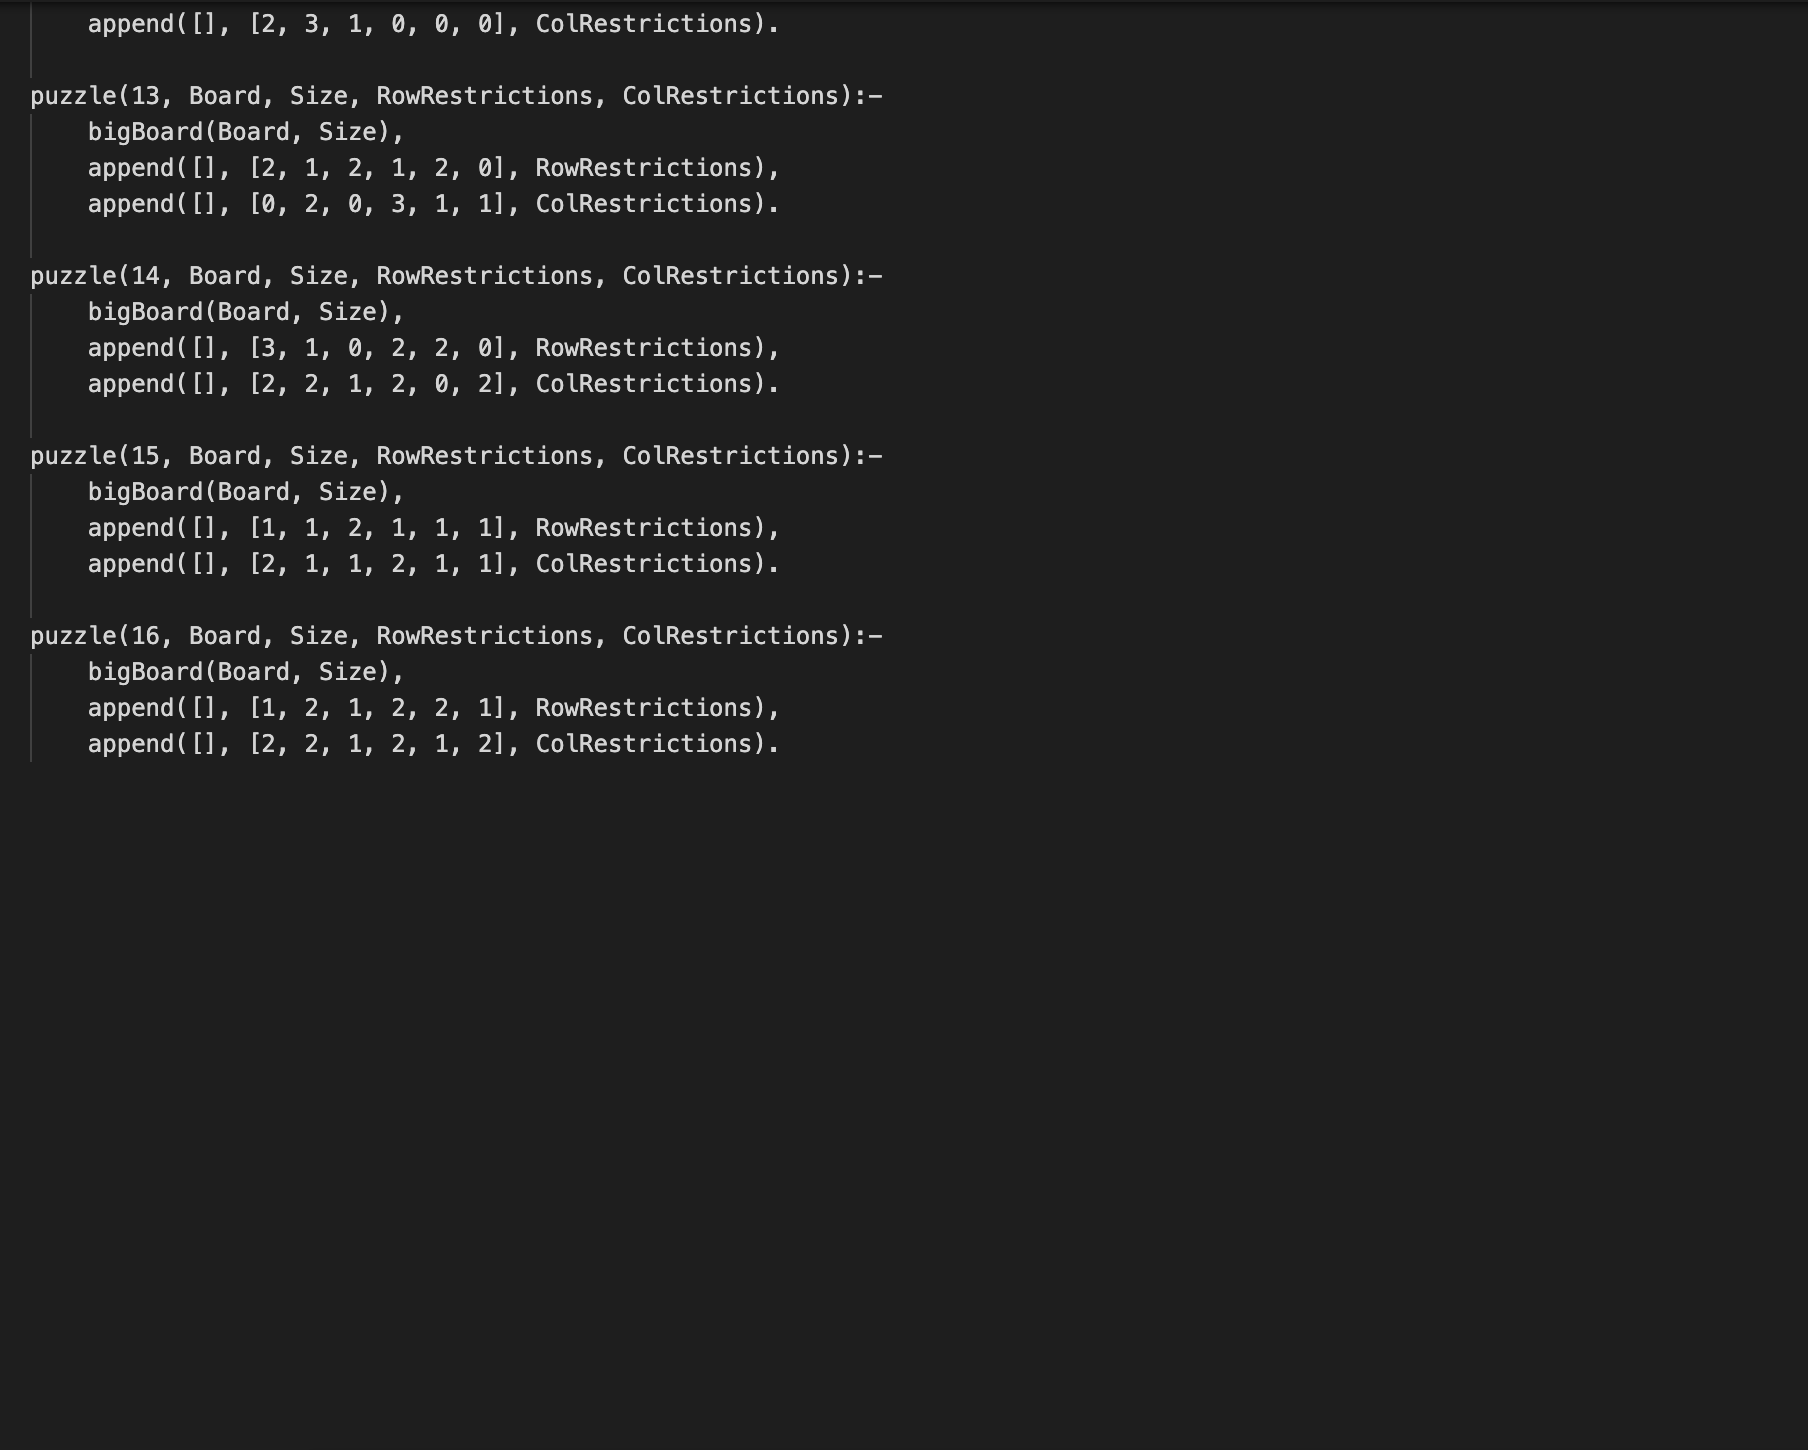
\includegraphics[scale=0.4]{img/20.png}
\end{center}

\subsection{display.pl}
\begin{center}
    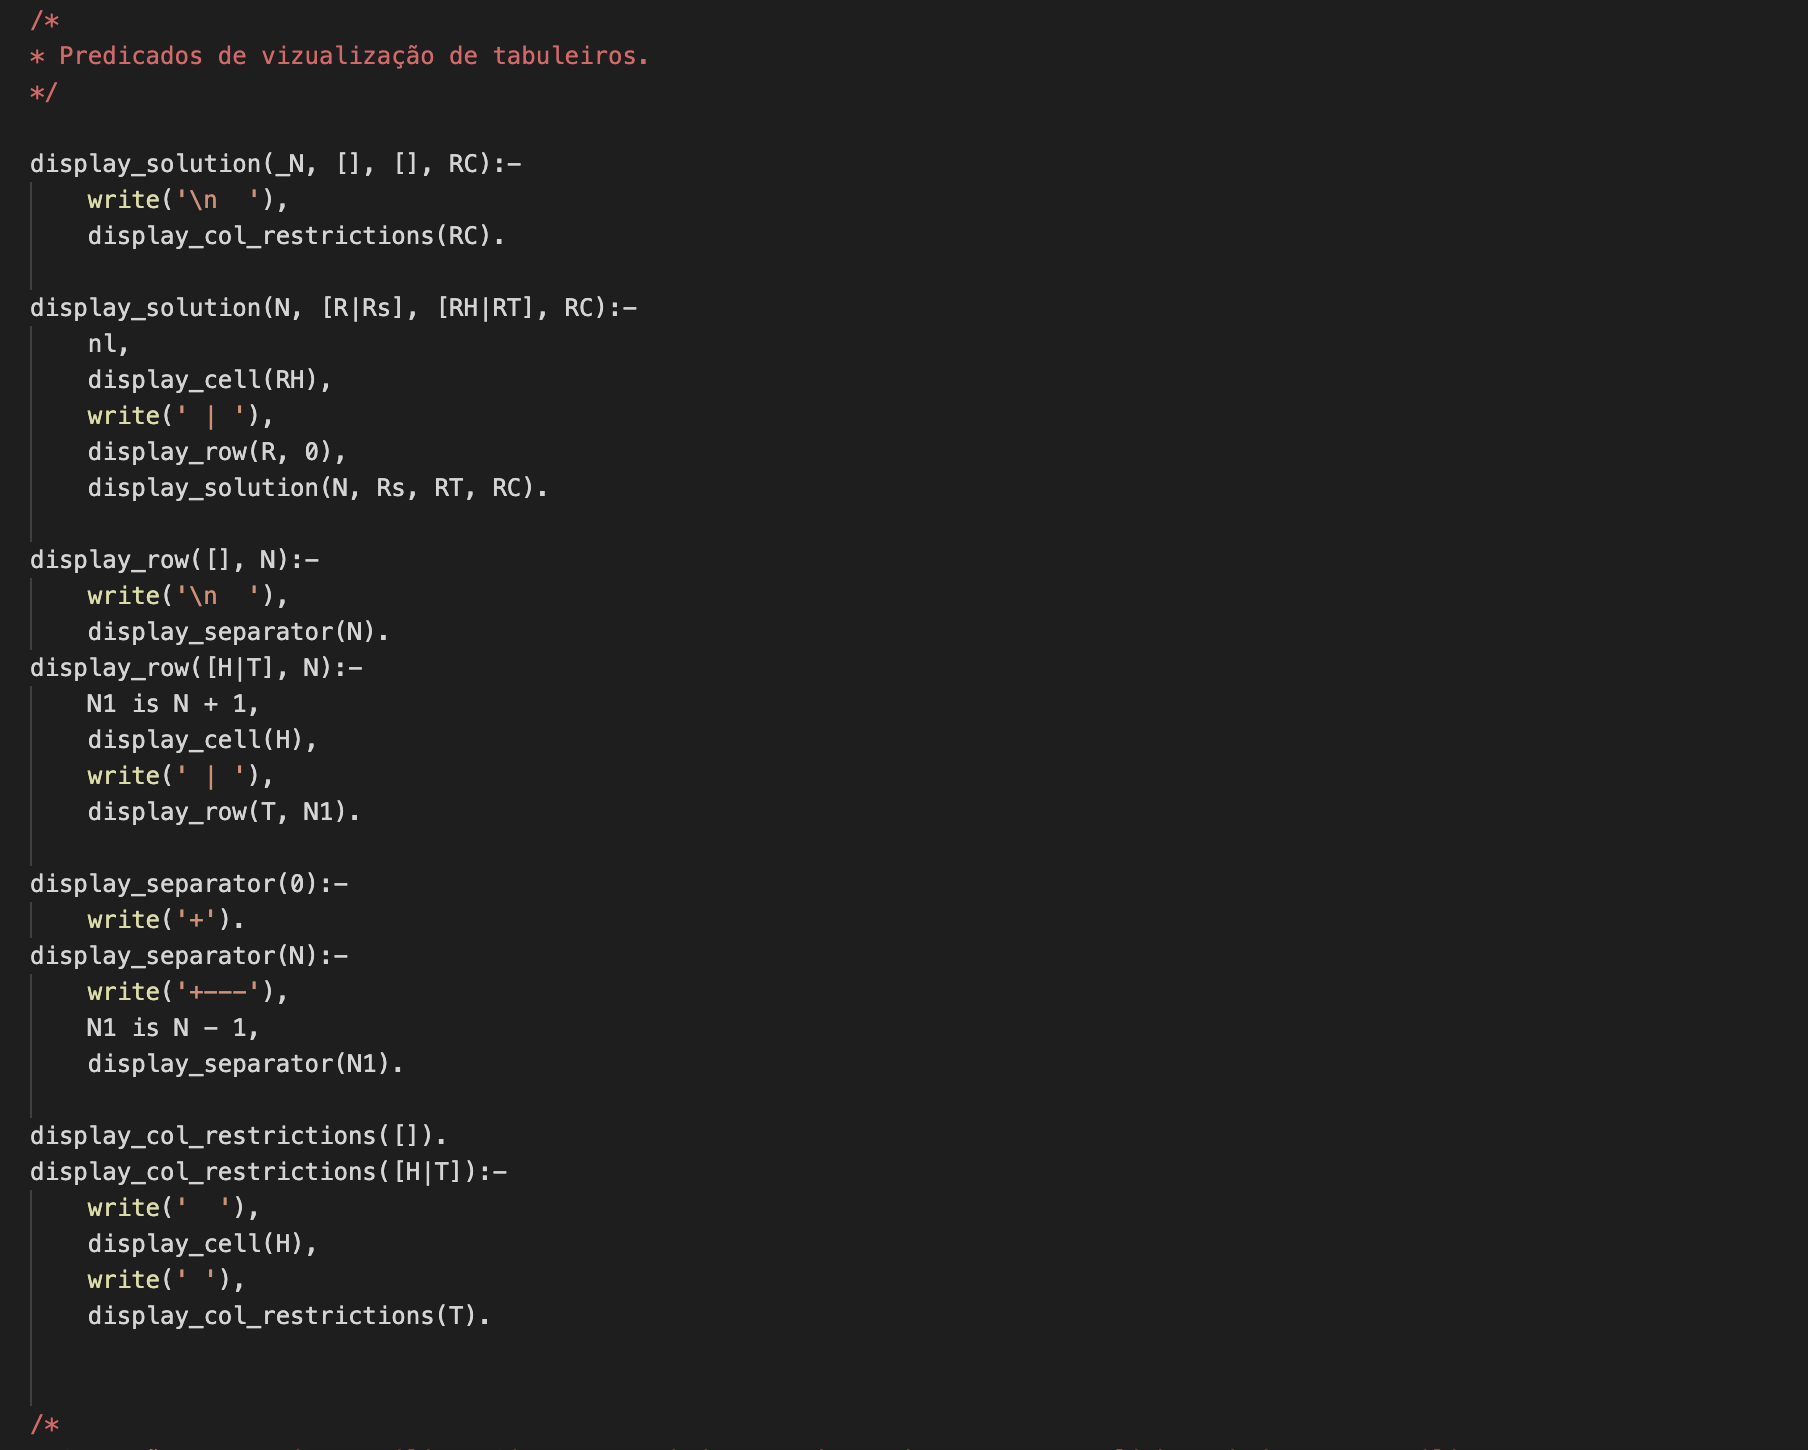
\includegraphics[scale=0.4]{img/21.png}
    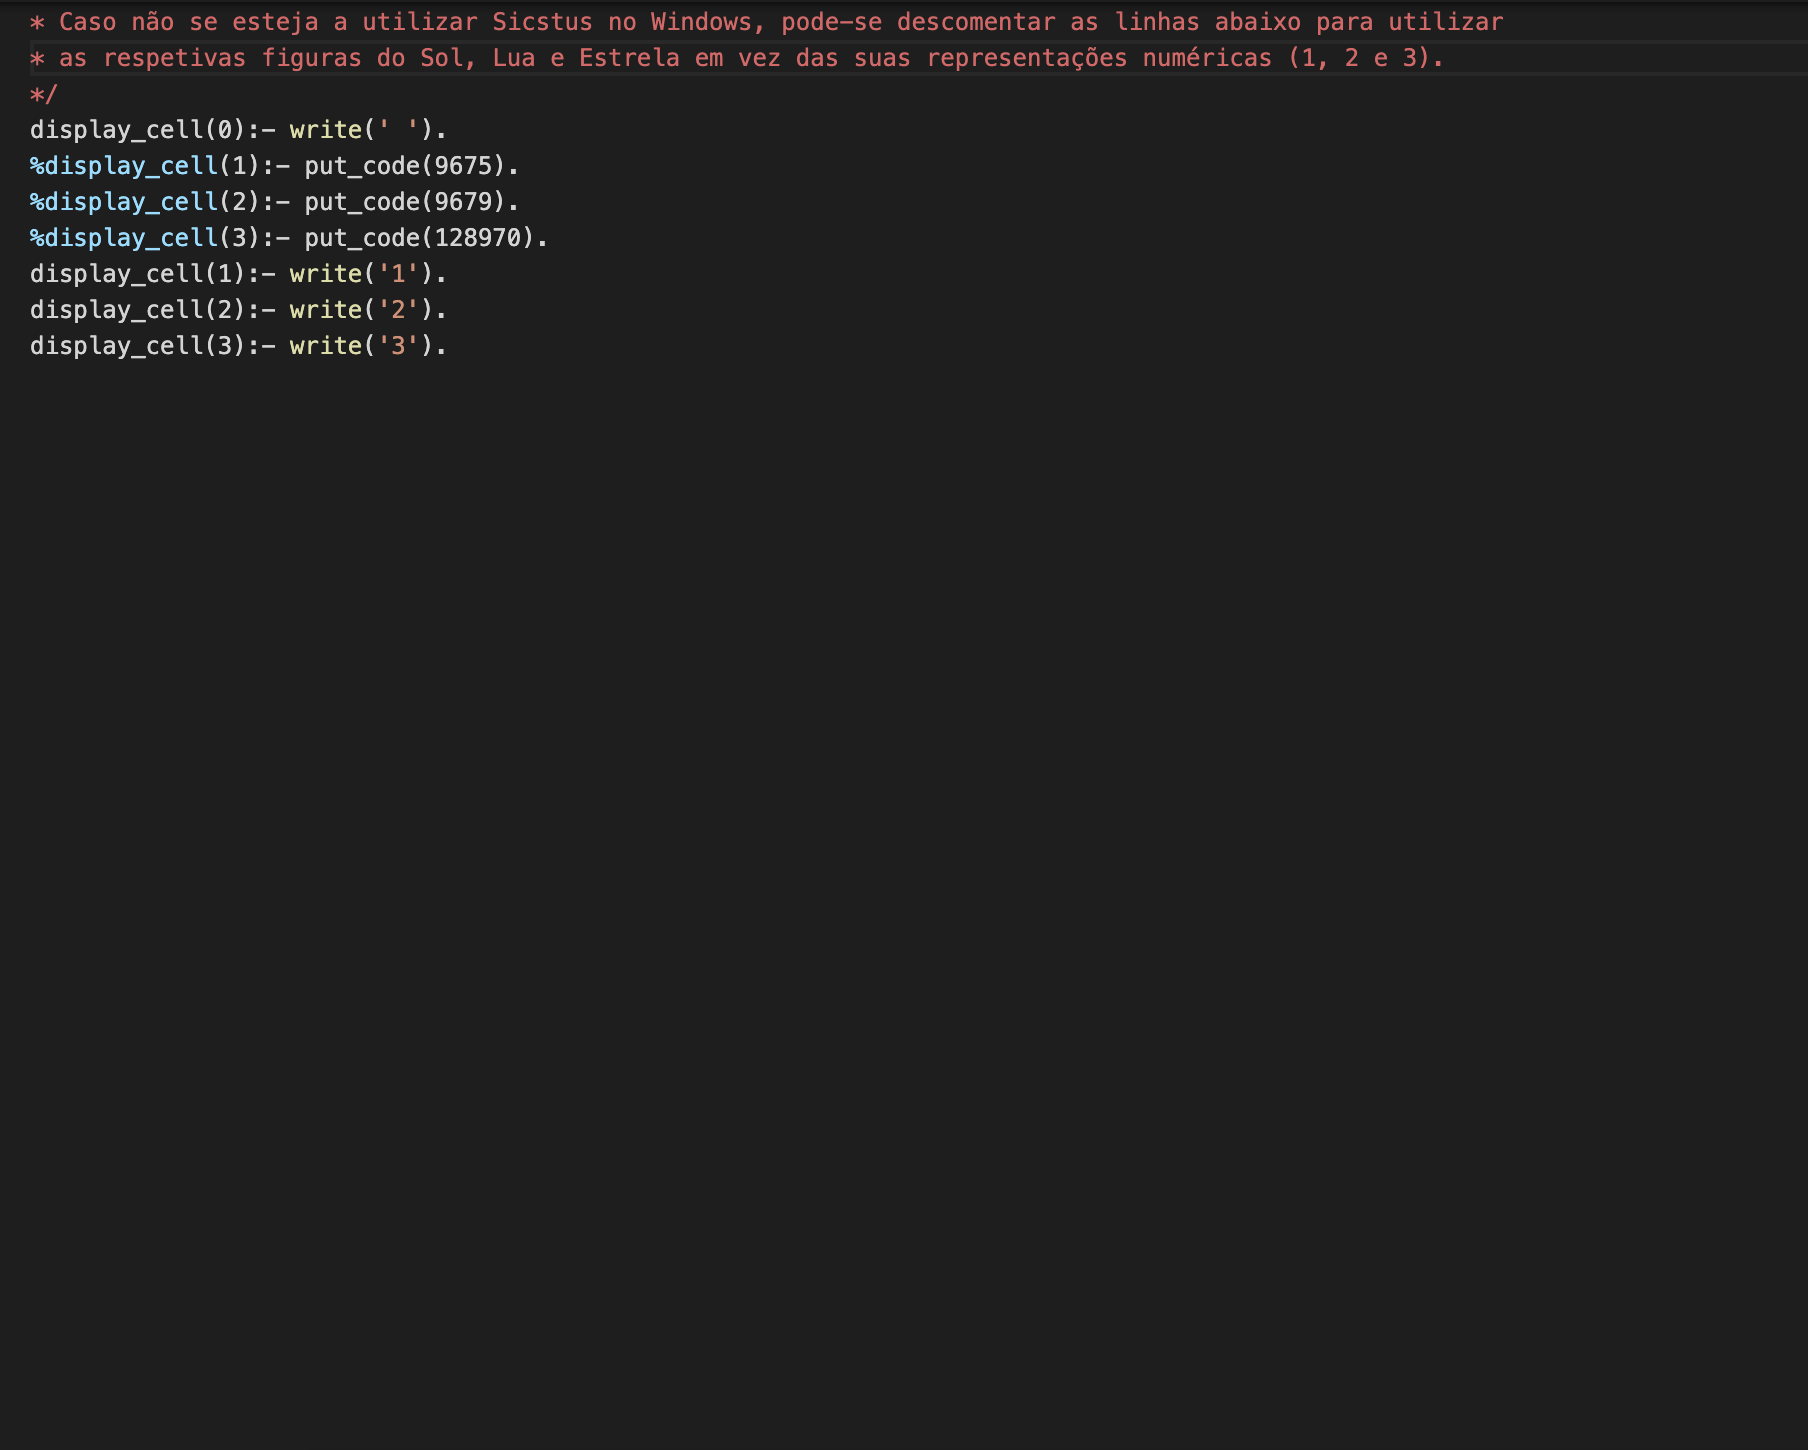
\includegraphics[scale=0.4]{img/22.png}
\end{center}

\subsection{utils.pl}
\begin{center}
    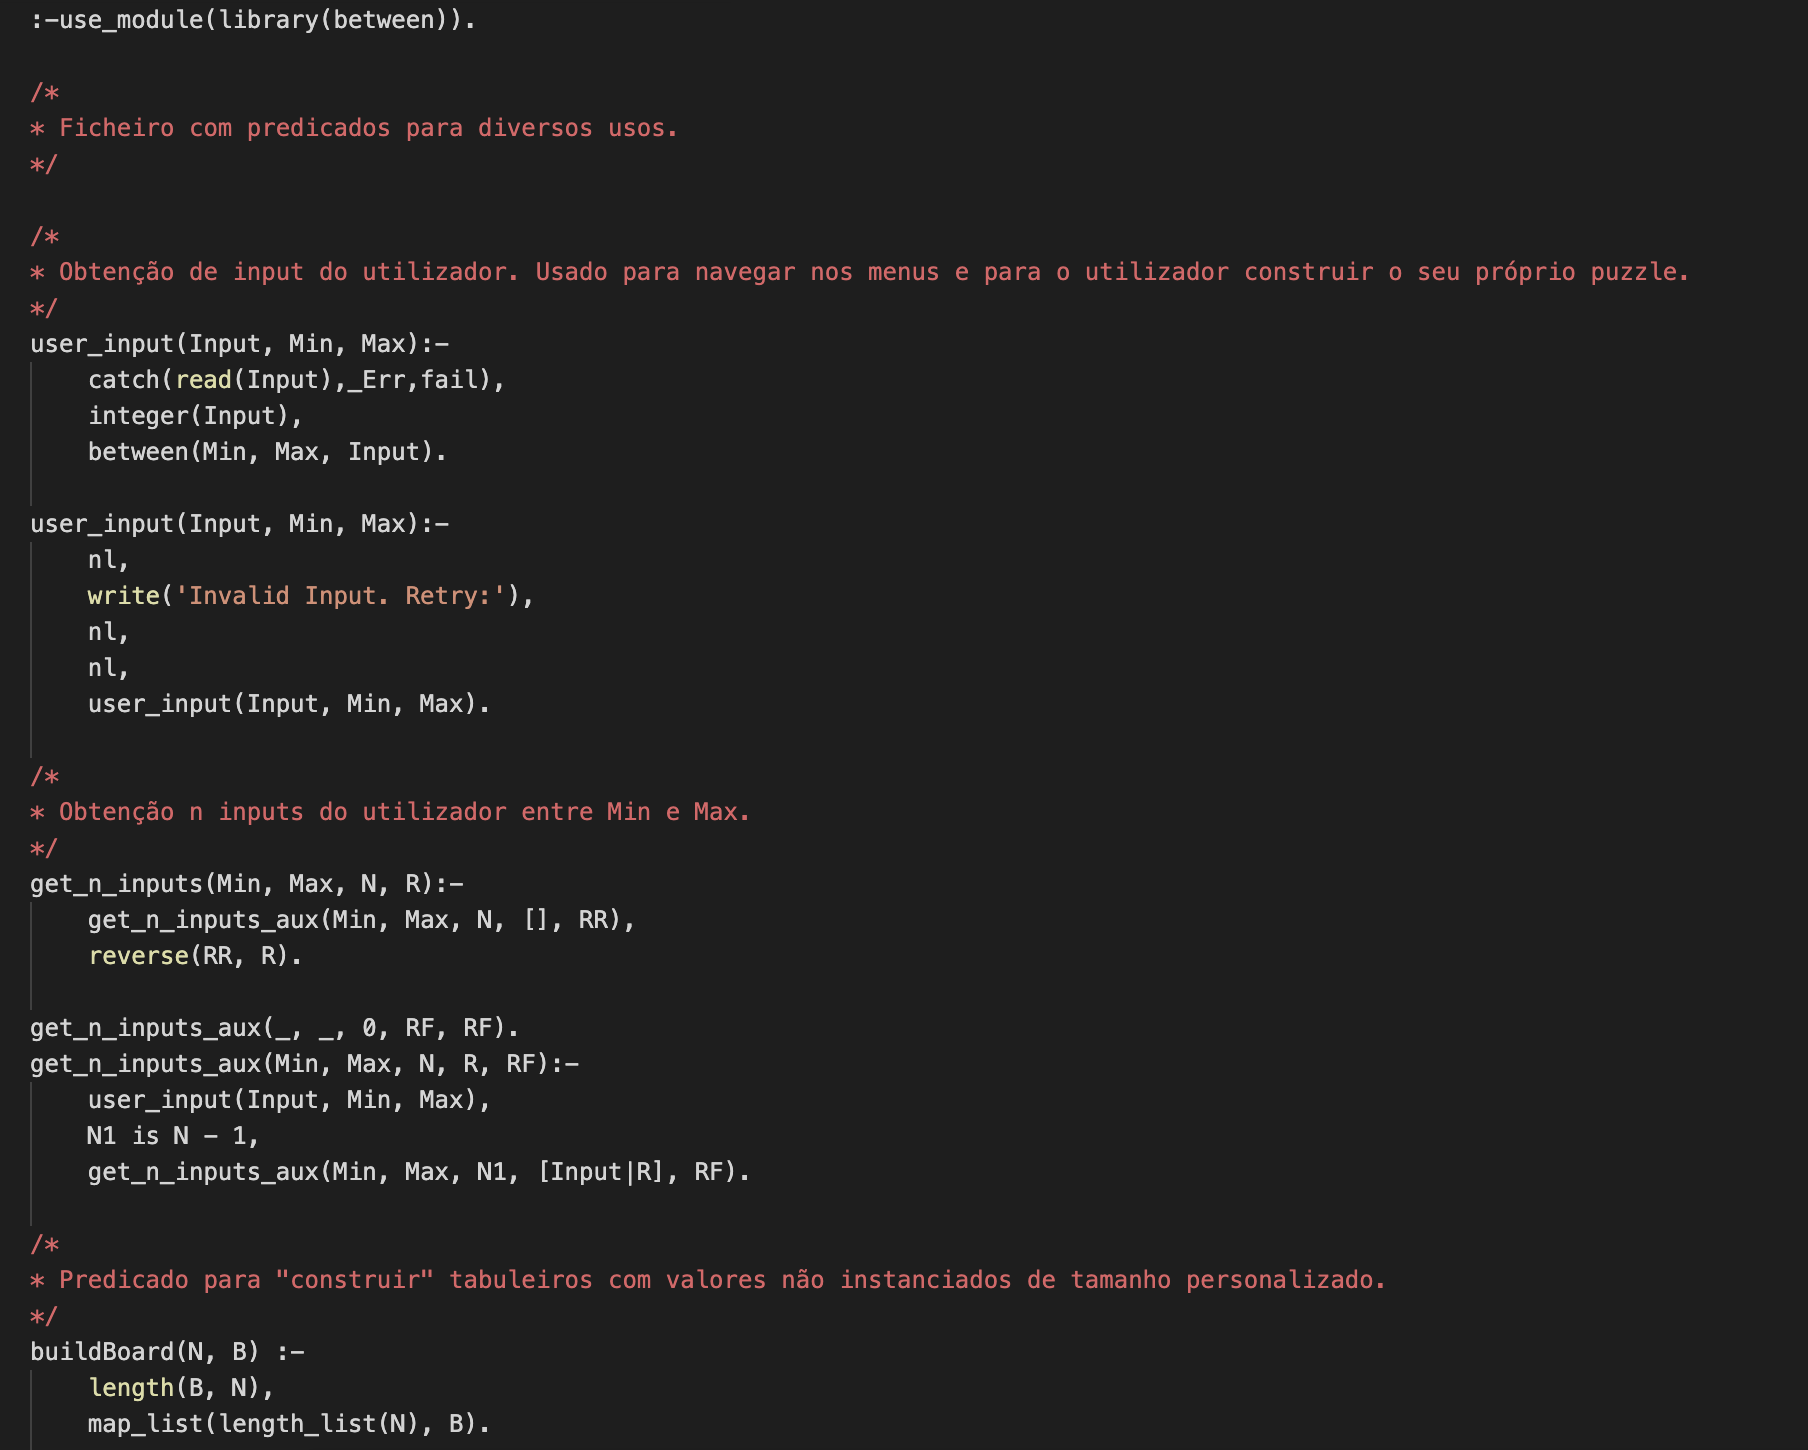
\includegraphics[scale=0.4]{img/23.png}
    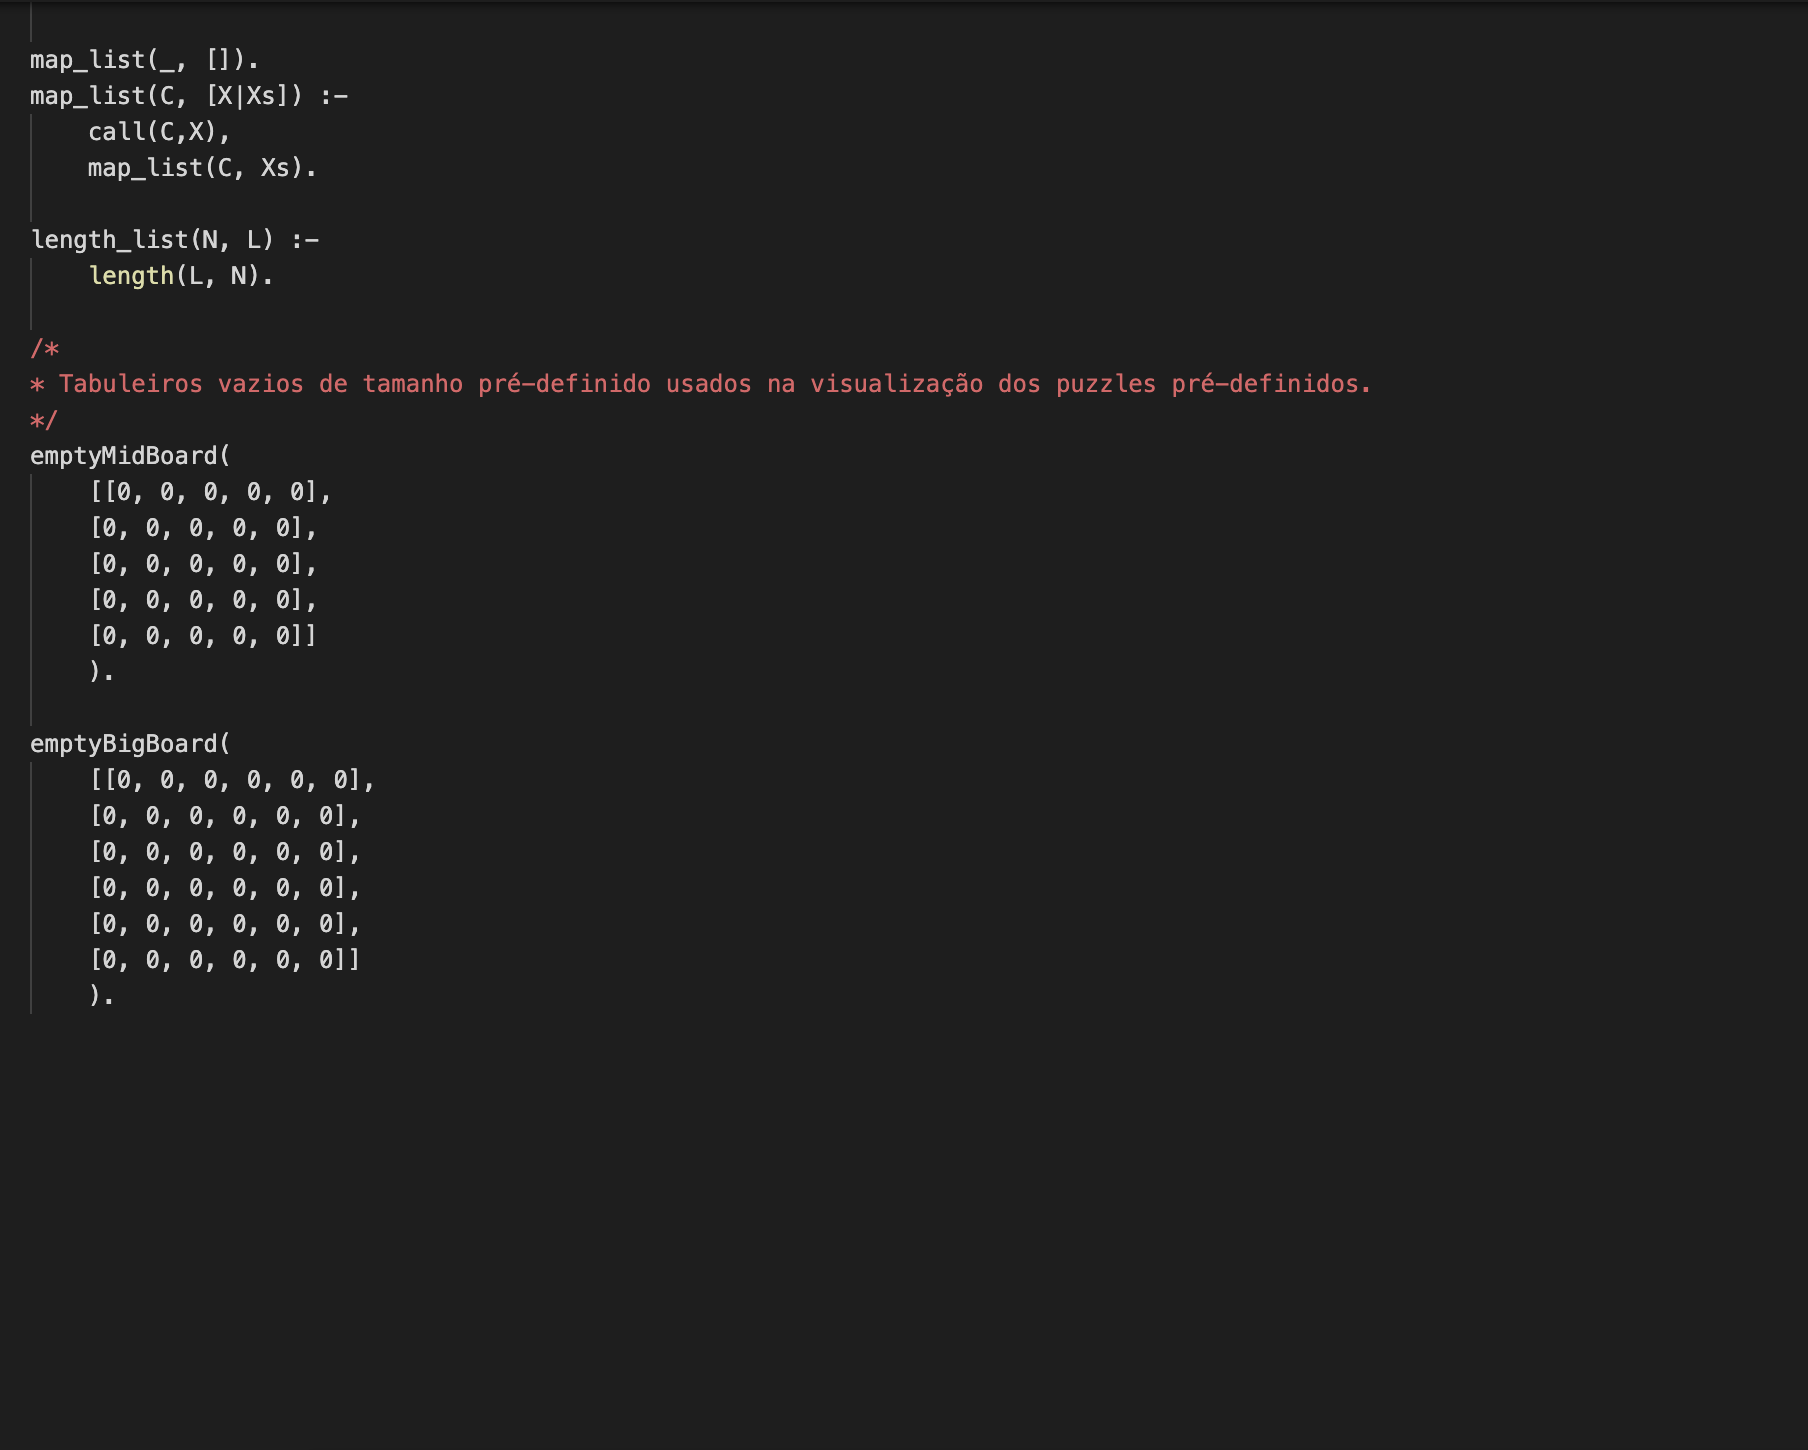
\includegraphics[scale=0.4]{img/24.png}
\end{center}

\clearpage
%\addcontentsline{toc}{section}{Bibliografia}
\renewcommand\refname{Apendix}
\bibliographystyle{apalike}
\bibliography{myrefs}

\newpage
\appendix
% \section{Nome do Anexo}
% Outros elementos úteis que não sejam essenciais ao relatório.

\end{document}